\documentclass[a4paper,zihao=5,UTF8]{ctexart}
\usepackage[top=2.3cm,bottom=2cm,left=1.7cm,right=1.7cm]{geometry} 
\usepackage{amsmath, amssymb}
\usepackage{color}
\usepackage{hyperref} 
\usepackage{pythonhighlight}
\usepackage{listings}
\usepackage{mathrsfs} 
\usepackage{booktabs}
\usepackage{amsthm}
\usepackage{longtable} 
\usepackage{graphicx}
\usepackage{subfigure}
\usepackage{caption}
\usepackage{fontspec}
\usepackage{titlesec}
\usepackage{fancyhdr}
\usepackage{latexsym}
\usepackage{braket}
\usepackage{cite}
\usepackage[version=4]{mhchem}
\usepackage{makecell}
\usepackage{listings}

\lstset{
 columns=fixed,       
 numbers=left,                                        % 在左侧显示行号
 numberstyle=\tiny\color{gray},                       % 设定行号格式
 frame=none,                                          % 不显示背景边框
 backgroundcolor=\color[RGB]{245,245,244},            % 设定背景颜色
 keywordstyle=\color[RGB]{40,40,255},                 % 设定关键字颜色
 numberstyle=\footnotesize\color{darkgray},           
 commentstyle=\it\color[RGB]{0,96,96},                % 设置代码注释的格式
 stringstyle=\rmfamily\slshape\color[RGB]{128,0,0},   % 设置字符串格式
 showstringspaces=false,                              % 不显示字符串中的空格
 language=c++,                                        % 设置语言
}

\CTEXsetup[format={\Large\bfseries}]{section}
\def\d{\mathrm{d}}
\def\e{\mathrm{e}}
\def\i{\mathrm{i}}
\def\dps{\displaystyle}
\newcommand{\mr}[1]{\mathrm{#1}}
\newcommand{\mb}[1]{\mathbf{#1}}
\newcommand{\dv}[2]{\frac{\d{#1}}{\d{#2}}}
\newcommand{\pdv}[2]{\frac{\partial{#1}}{\partial{#2}}}
\def\degree{$^{\circ}$}
\def\celsius{^{\circ}\mr{C}}
\title{\textbf{绝热不变量}}
\author{王崇斌\;1800011716}
\makeatletter
\makeatother
\begin{document}
	\pagestyle{fancy}
	\pagestyle{fancy}
    \lhead{计算物理A}
	\chead{}
	\rhead{\today}
	\maketitle
    \thispagestyle{fancy}
    \tableofcontents
    \section{题目描述}
    对于单自由度非含时Hamilton系统, 总可以定义绝热不变量\ref{def of J}, 它表示了相轨迹在相空间中包围的面积:
    \begin{equation}
        J := \frac{1}{2\pi}\oint p\d q
        \label{def of J}
    \end{equation}
    可以直接计算出$J$的显式表达式\ref{explicit J}:
    \begin{equation}
        J = \frac{1}{\pi}\int_{q_{\mr{min}}}^{q_{\mr{max}}}\sqrt{2m[E - V(q)]}\d q
        \label{explicit J}
    \end{equation}
    系统的周期可以表示为能量$E$的函数\ref{explicit periodic}:
    \begin{equation}
        T = \int_{q_{\mr{min}}}^{q_{\mr{max}}}\sqrt{\frac{2m}{E - V(q)}} \d q
        \label{explicit periodic}
    \end{equation}
    那么可以看出绝热不变量$J$与周期$T$之间的关系\ref{relation J E}:
    \begin{equation}
        \dv{J}{E} = \frac{T}{2\pi}
        \label{relation J E}
    \end{equation}
    若哈密顿量中存在随时间缓慢改变的参数$\lambda(t)$, 绝热定理宣称在参数缓慢改变时, 绝热不变量
    基本不随参数变化\ref{adiabatic theorem}:
    \begin{equation}
        \lim_{\d \lambda / \d t \to 0}\dv{I}{\lambda} = 0
        \label{adiabatic theorem}
    \end{equation}
    在本题中通过研究一个力学系统的长期行为来讨论绝热不变量的适用性.
    系统的哈密顿量为\ref{Hamiltonian}:
    \begin{equation}
        H(p_y, y) = \frac{p_y^2}{2m} + \frac{1}{2}k\left(\sqrt{x^2 + y^2} - l\right)^2 + mgy
        \label{Hamiltonian}
    \end{equation}
    \section{问题}
    \subsection{系统的平衡位置}
    首先形象地理解一下$x, g$两个参数对于系统势能的影响, 当$x$从大变小时
    (此时假设$g=0$), 系统的势能会逐渐从一个单势阱变为双势阱, 在$y=0$处产生了一个势能极大值点. 
    这其中经历了势能函数凹凸性的变化, 即存在二阶导数从恒正变为有正有负. 当二阶导数变号时势能函数存在拐点
    (二阶导数为0), 在两个拐点之间函数凹凸性一致, \textbf{如果}两个拐点处势能函数的导数值符号相反, 
    这意味着两个拐点之间存在唯一的极值点, 结合实际情况, 只可能存在势能极大值点(
    后面会利用这个性质来选择给定总能量情况下数值求解经典拐点时初始猜测的区间), 这时极大值点两侧一定存在两个
    势能极小值点, 对应系统的两个稳定平衡位置. 当$g\neq 0$时, 相当于在双势阱的基础上加上了一个线性的势能, 
    产生的结果使双势阱不再对称, 势能如果存在极大值点也不会在$y=0$处, 但是拐点的存在性和位置与新加上的线性
    势能无关, 因此两个拐点之间依然有可能存在局域极大值, 存在的判据与前一段论述相同. 考虑一个
    临界情况, 当线性势能变强的过程中, 某一侧势阱的极小值点会“渐渐消失”, “恰好消失”对应了\textbf{势能极小值点
    与拐点重合的情况}. 计算势能函数的导数与二阶导数为:
    \begin{equation}
        \left\{
            \begin{aligned}
                \dv{V}{y} &= ky\left(1 - \frac{l}{\sqrt{x^2 + y^2}}\right) + mg\\
                \dv{^2V}{y^2} &= k\left(1 - \frac{lx^2}{(x^2 + y^2)^{3/2}}\right)
            \end{aligned}
        \right.
    \end{equation}
    可以看出拐点的存在与否与$g$无关, 拐点存在当且仅当$0 < x < l$, 拐点为:
    \begin{equation}
        y^*_{\pm} = \pm x\sqrt{\left(\frac{l}{x}\right)^{2/3} - 1}
    \end{equation}
    将上面的表达式带入势能导数的表达式并令其等于0:
    \begin{equation}
        \pm kx\sqrt{\left(\frac{l}{x}\right)^{2/3} - 1}\left[1 - \left(\frac{l}{x}\right)^{2/3}\right] + mg = 0
    \end{equation}
    不妨假设$g>0$, 同时考虑$0 < x< l$, 可知上式中只能取+, 化简上式可以给出系统在包含一个稳定平衡点和包含
    两个稳定平衡点的分界线(分界线对应系统有一个随遇平衡点):
    \begin{equation}
        \left(\frac{l}{x}\right)^{2/3} = 1 + \left(\frac{mg}{kx}\right)^{2/3}\Leftrightarrow 
        1 = \left(\frac{x}{l}\right)^{2/3} + \left(\frac{mg}{kl}\right)^{2/3}
        \label{boundary}
    \end{equation}
    容易想象, 系统仅有一个极值点的情形对应:
    \begin{equation}
        1 < \left(\frac{x}{l}\right)^{2/3} + \left(\frac{mg}{kl}\right)^{2/3}
    \end{equation}
    将分界线\ref{boundary}绘制于图\ref{boundary figure}中:
    \begin{figure}
        \centering
        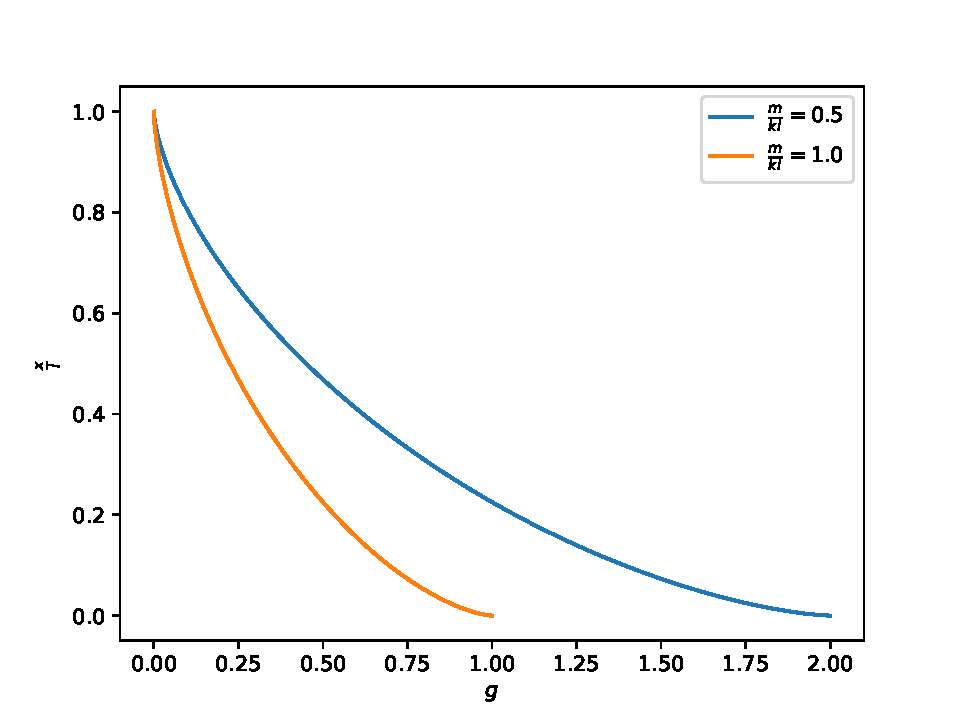
\includegraphics[scale=0.6]{1_boundary.pdf}
        \caption{系统存在一个稳定平衡点和两个稳定平衡点的分界线}
        \label{boundary figure}
    \end{figure} 
    \subsection{绝热不变量}
    这两问计算的程序参见2\_trajactory.cpp与3\_trajactory.cpp, 编译使用compile2.bat与compile3.bat, 
    可执行文件会生成一个储存了轨线等信息的文本文档, 相应的绘图程序参见2\_plot\_trajactory.py与
    3\_plot\_trajactory.py.
    \subsubsection{$x$作为缓变参数}
    为了方便起见, 将系统中的参数选为$m = 1, k = 1, l = 1$, 根据题目条件$g=0$.
    将对应了四种速度的相轨道绘制在表\ref{v change}中, 数值演化哈密顿方程采用了Velocity-Verlet算法
    (相应代码在2\_trajactory.cpp中):
    \begin{lstlisting}
        void Velocity_Verlet(double *x, double *p,
                     double (*f)(double *, double, double), double dt, double v,
                     double t) {
            double p1 = 0;
            p1 = p[0] + 0.5 * dt * f(x, v, t);
            x[0] = p1 / m * dt + x[0];
            p[0] = p1 + 0.5 * dt * f(x, v, t);}
    \end{lstlisting}
    \begin{table}[htbp]
        \centering
        \begin{tabular}[htbp]{cc}
            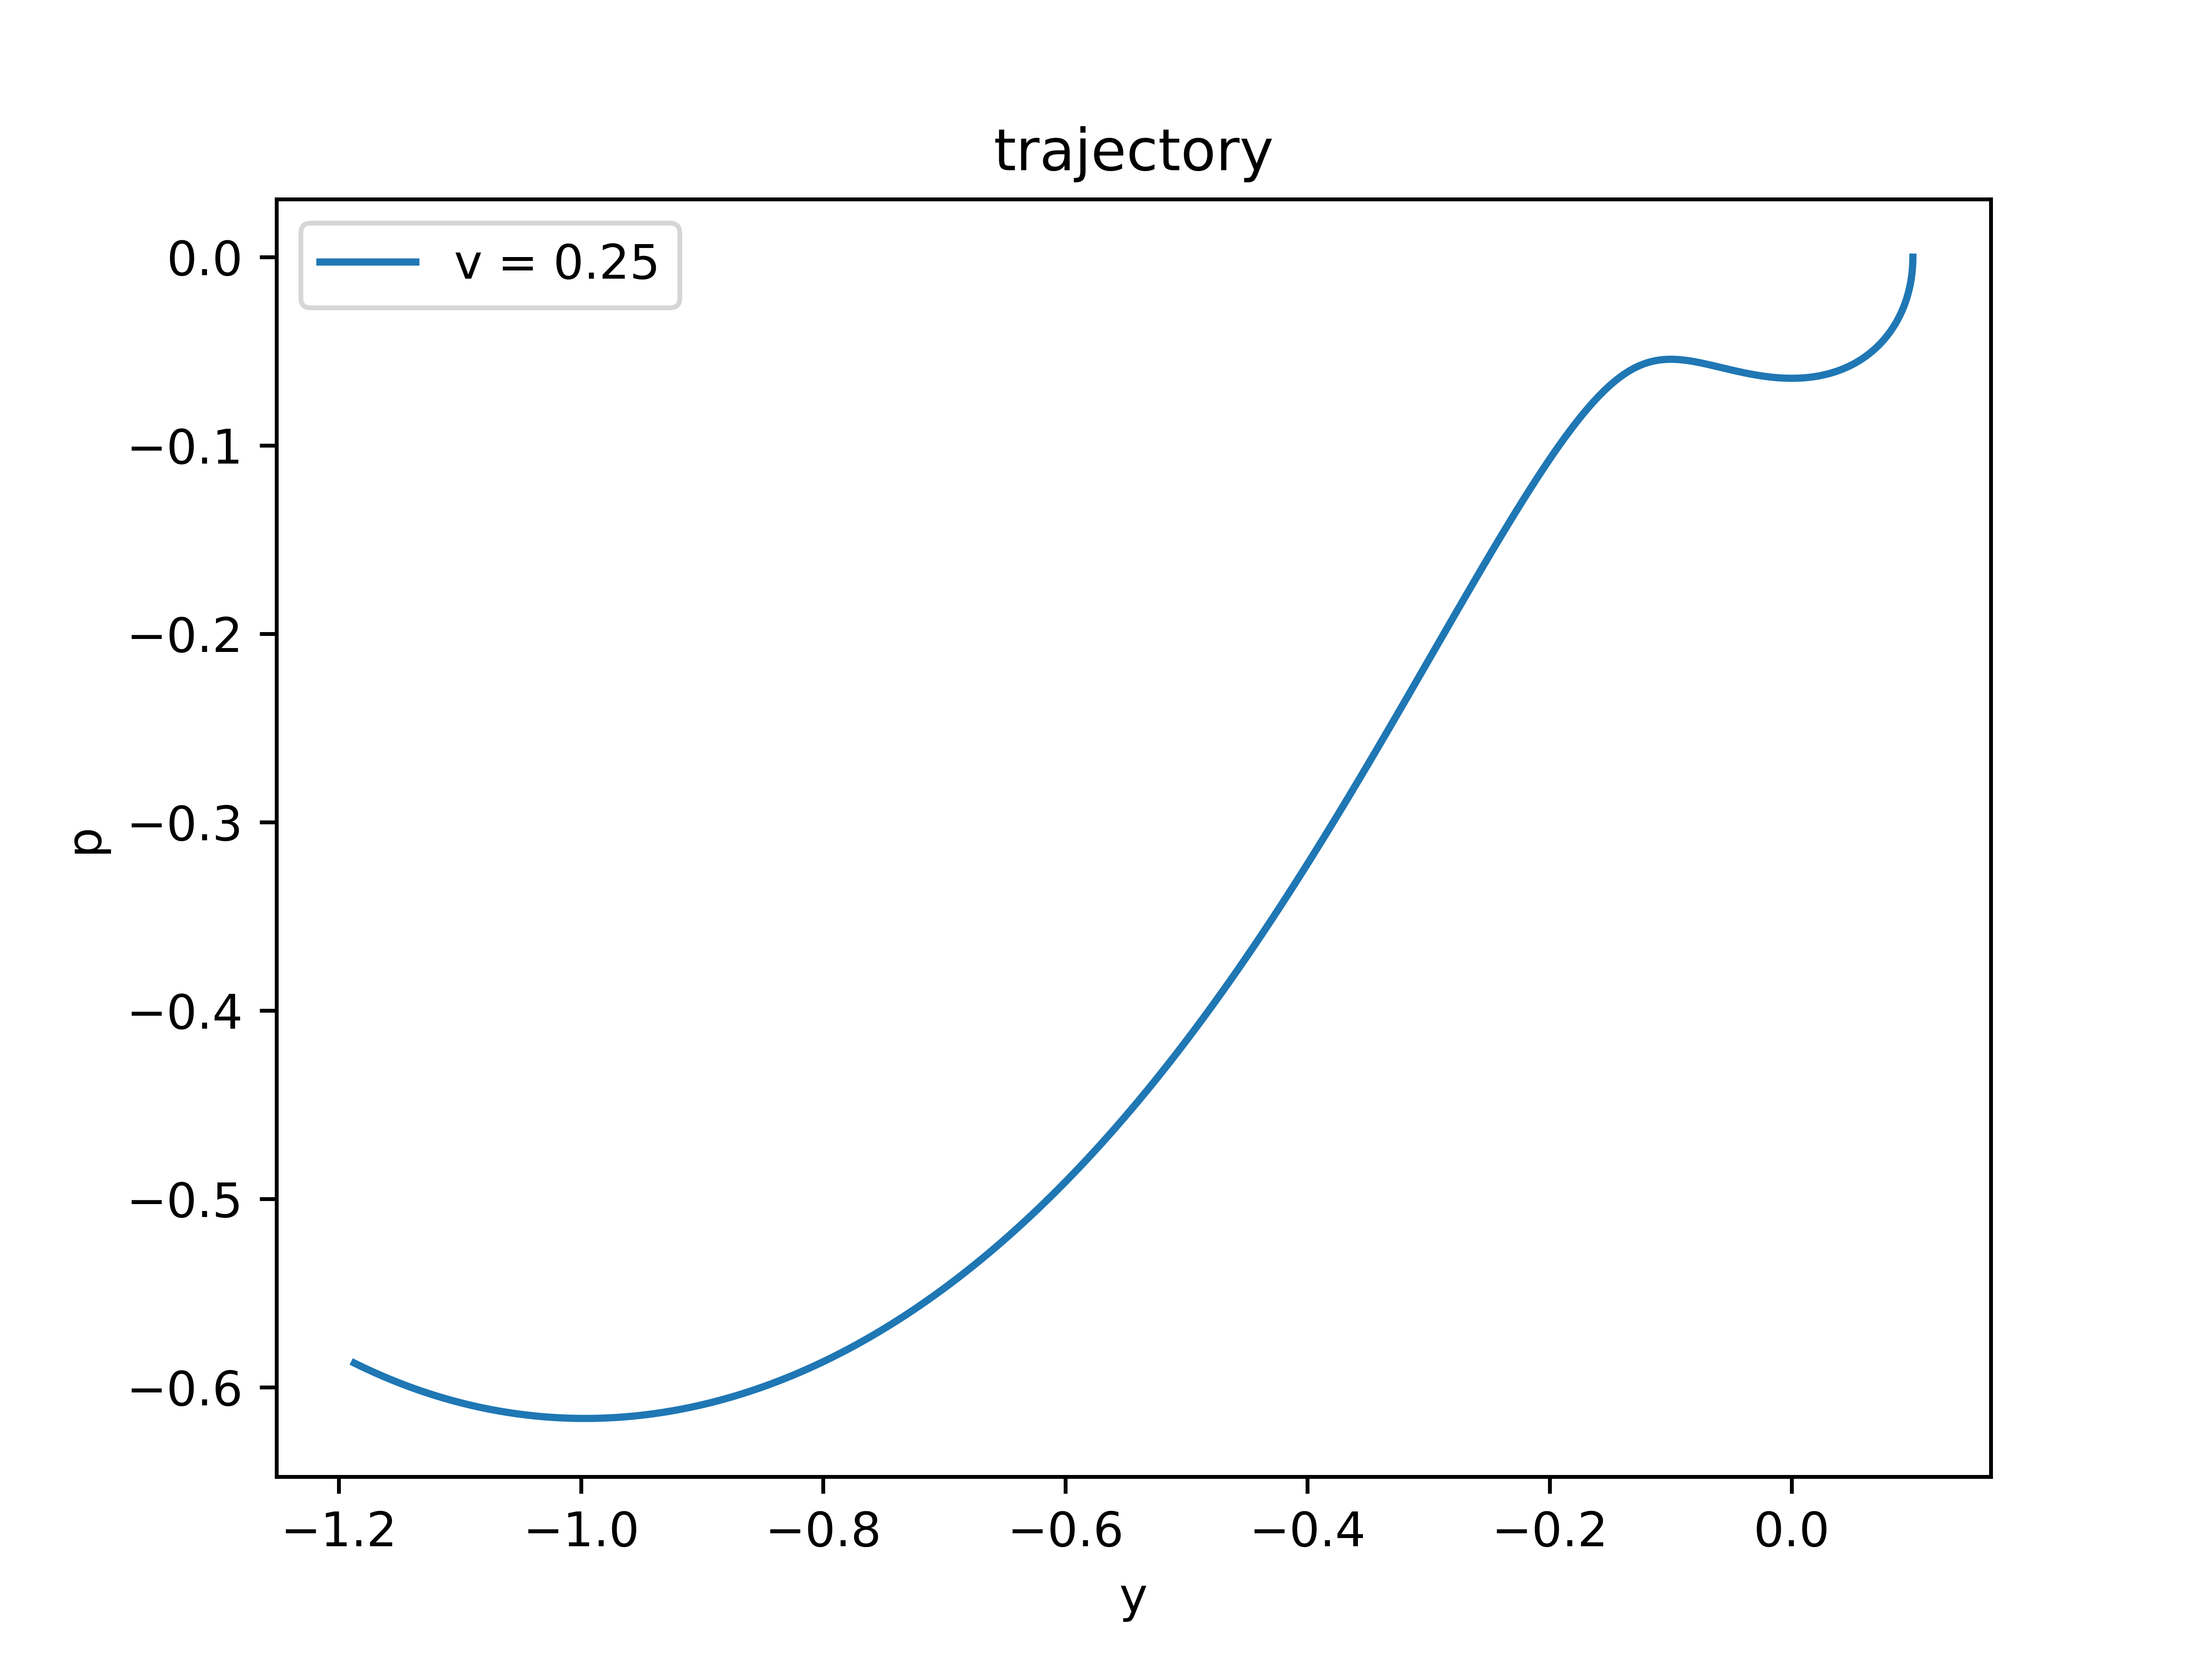
\includegraphics[scale=0.5]{2_traj_v=0_25.png} & 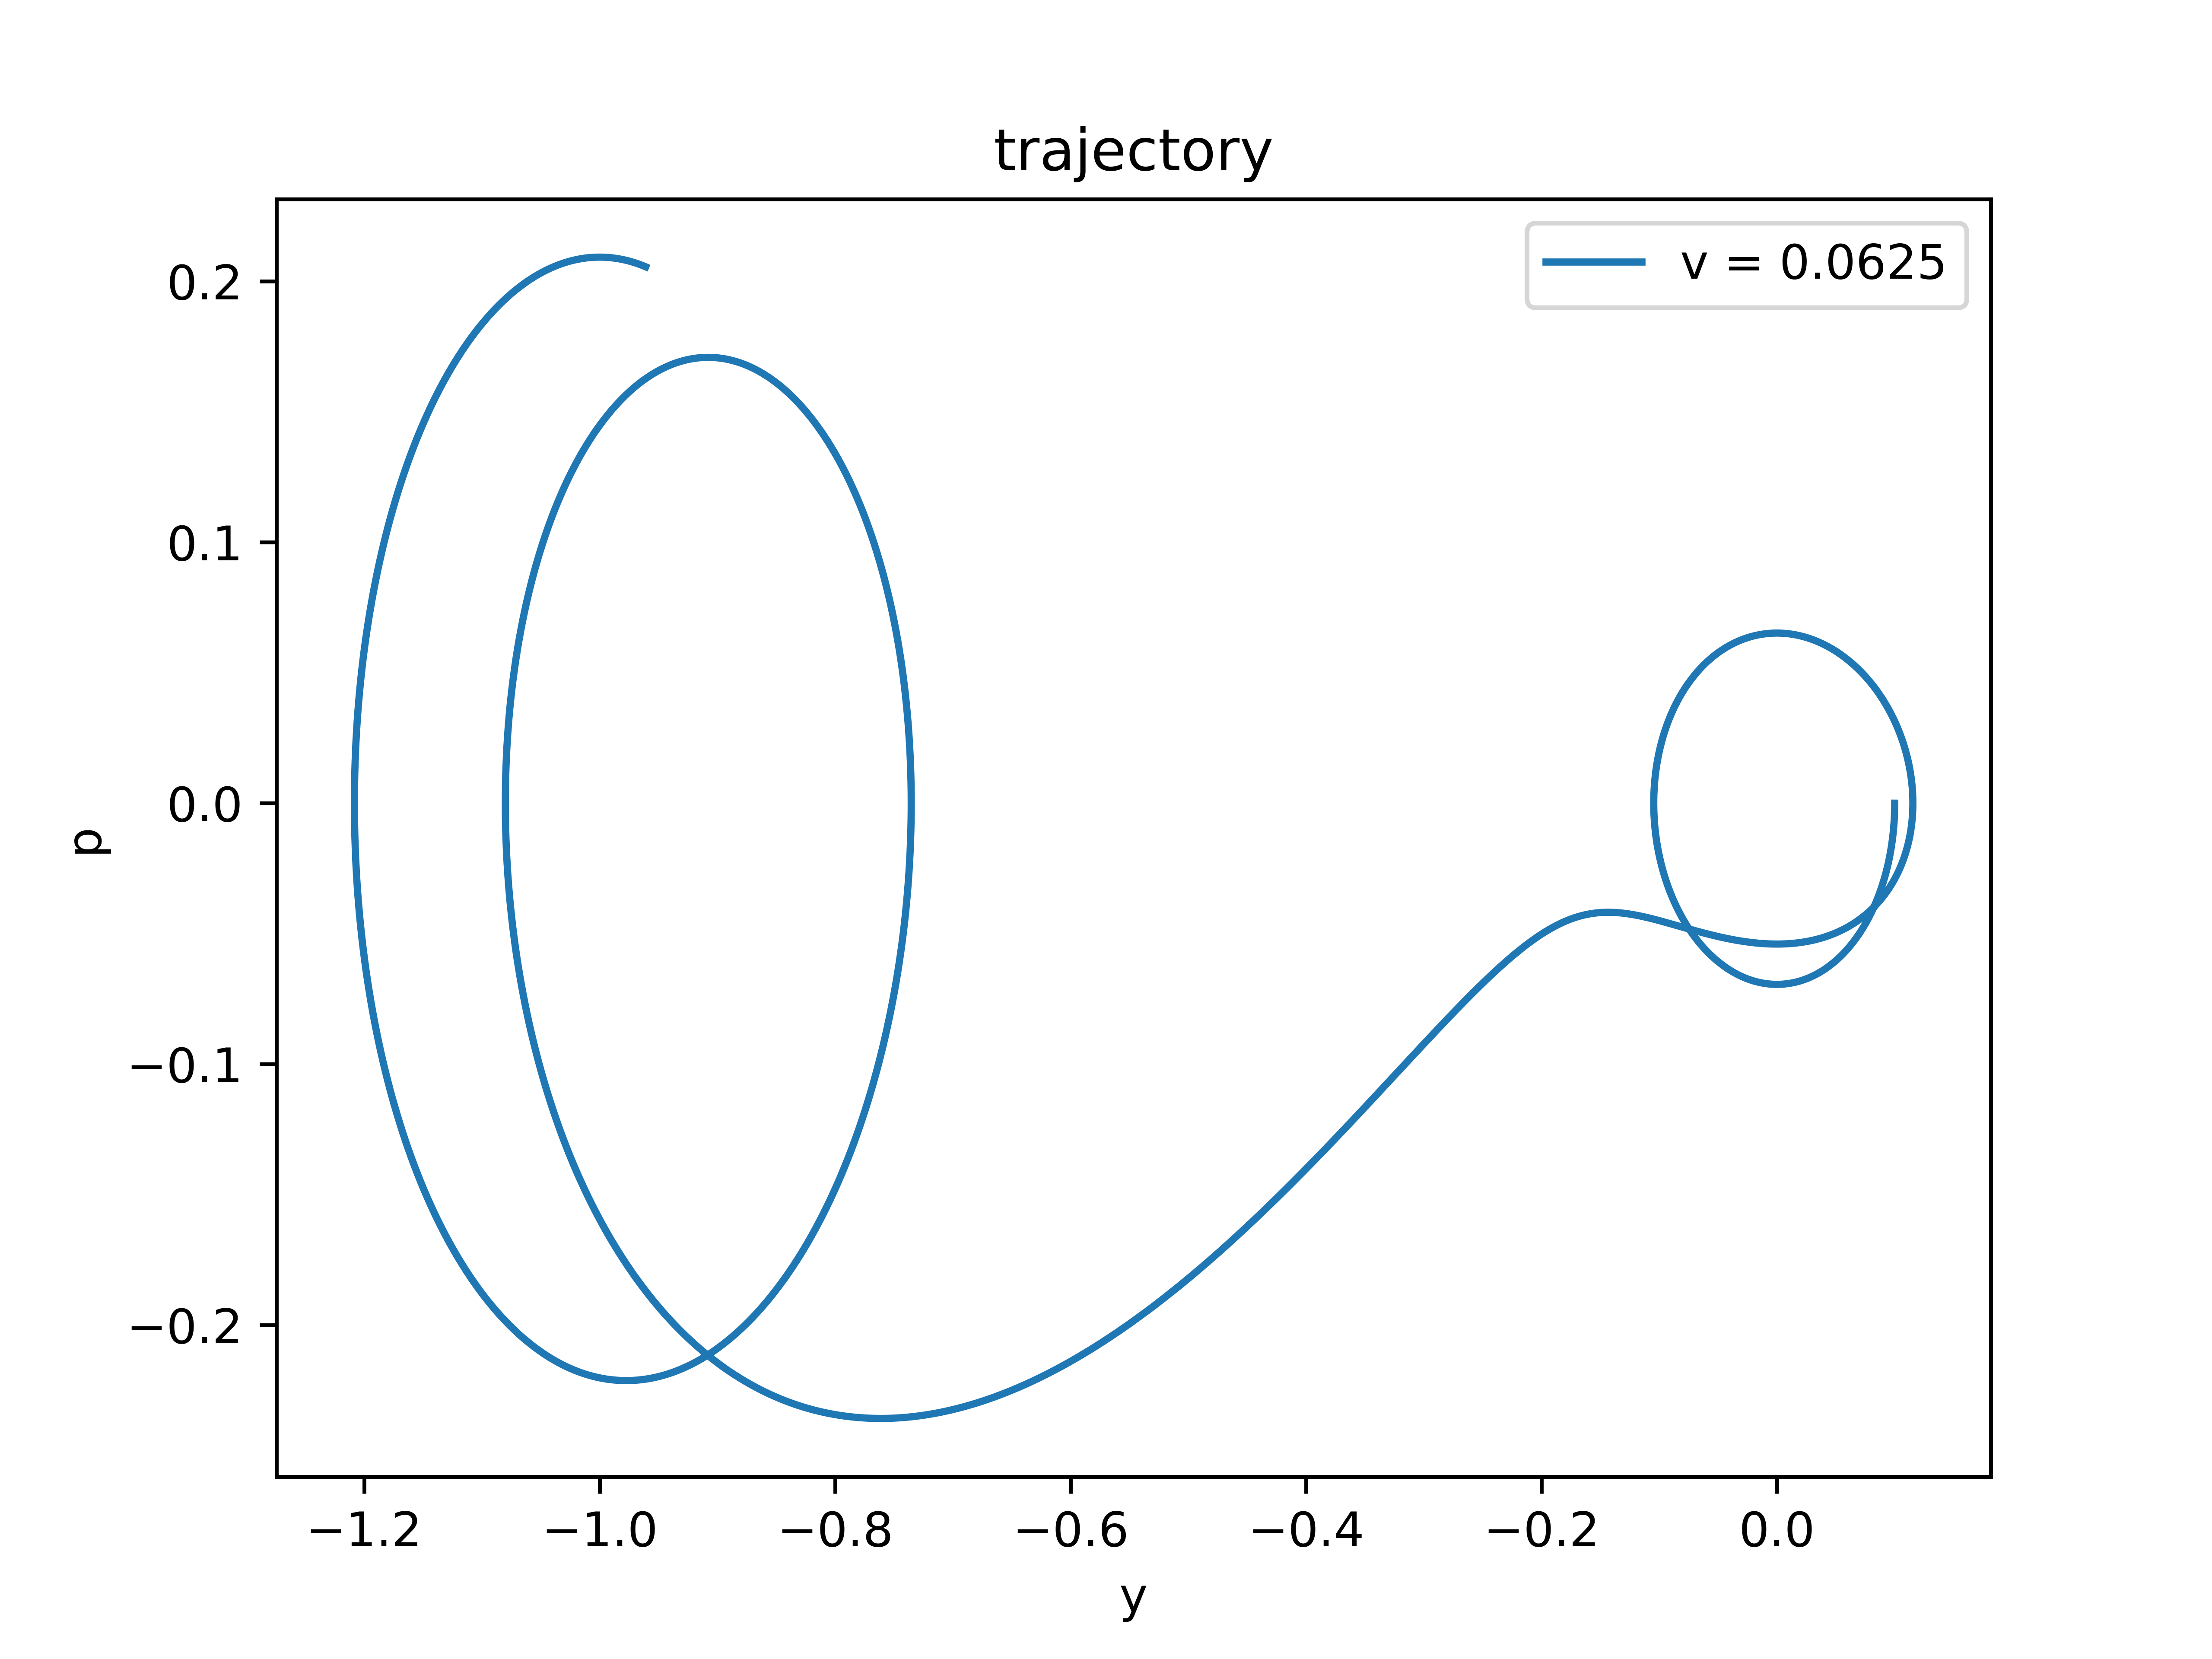
\includegraphics[scale=0.5]{2_traj_v=0_0625.png} \\
            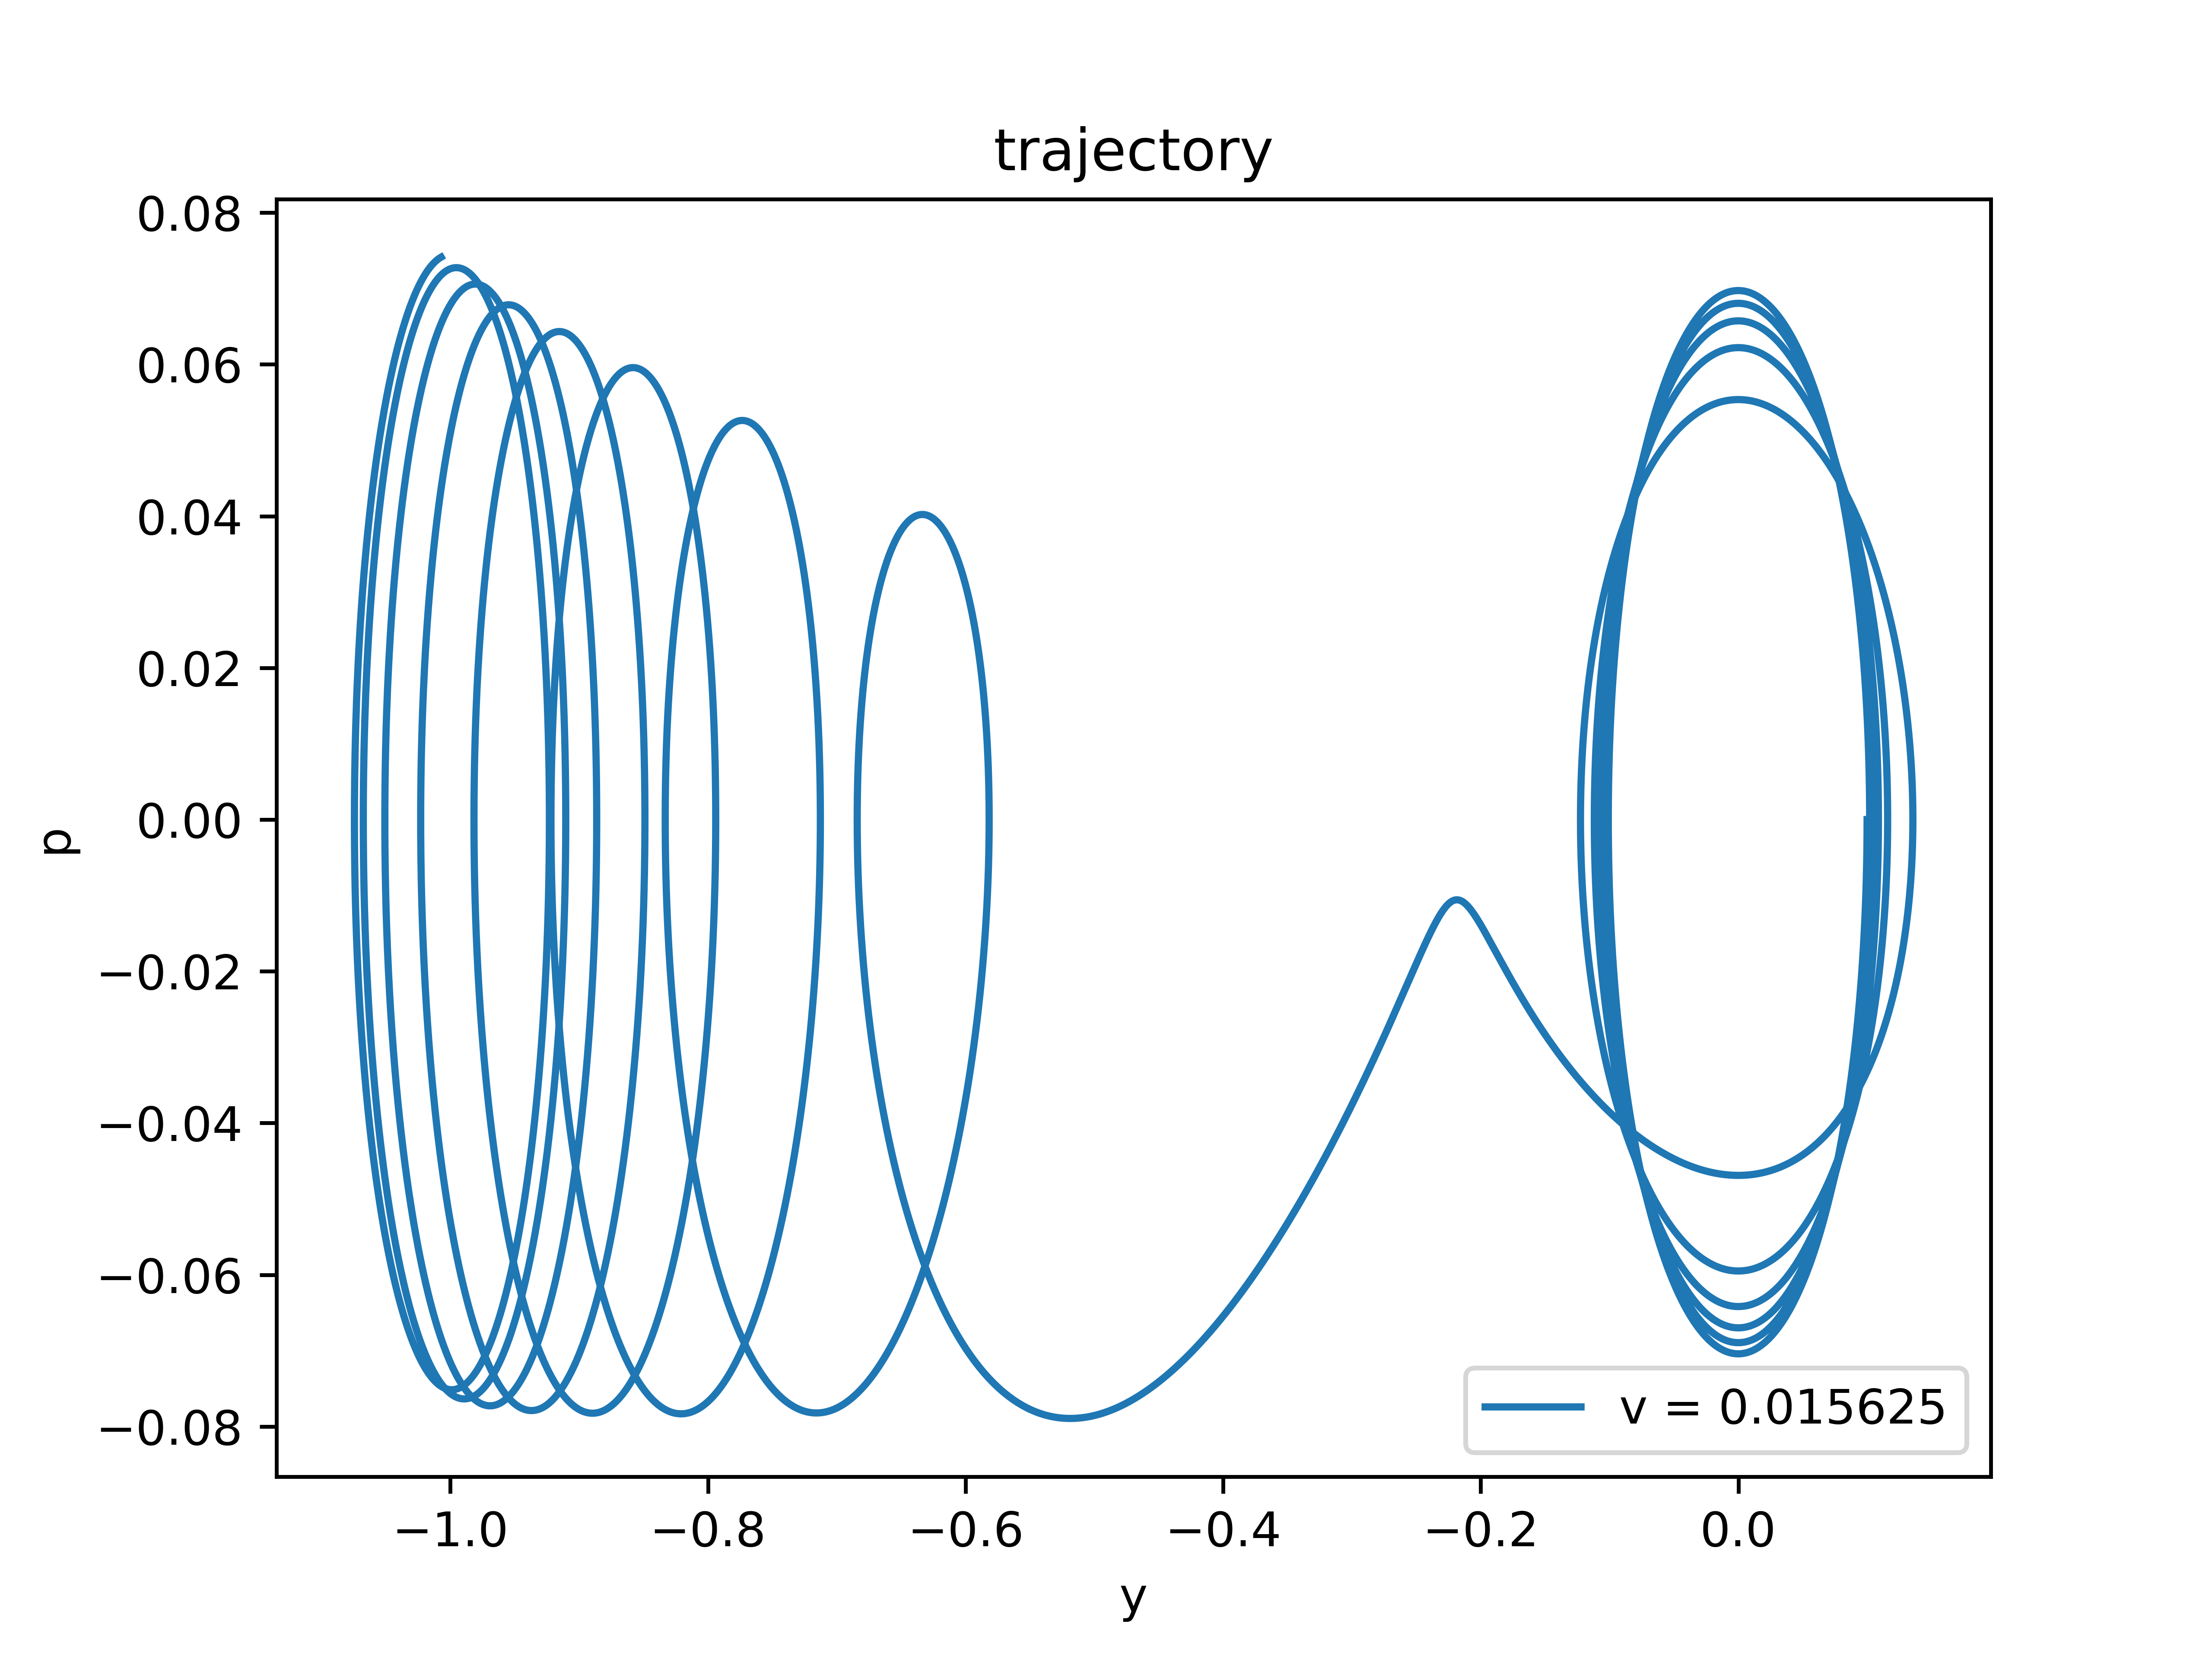
\includegraphics[scale=0.5]{2_traj_v=0_015625.png} & 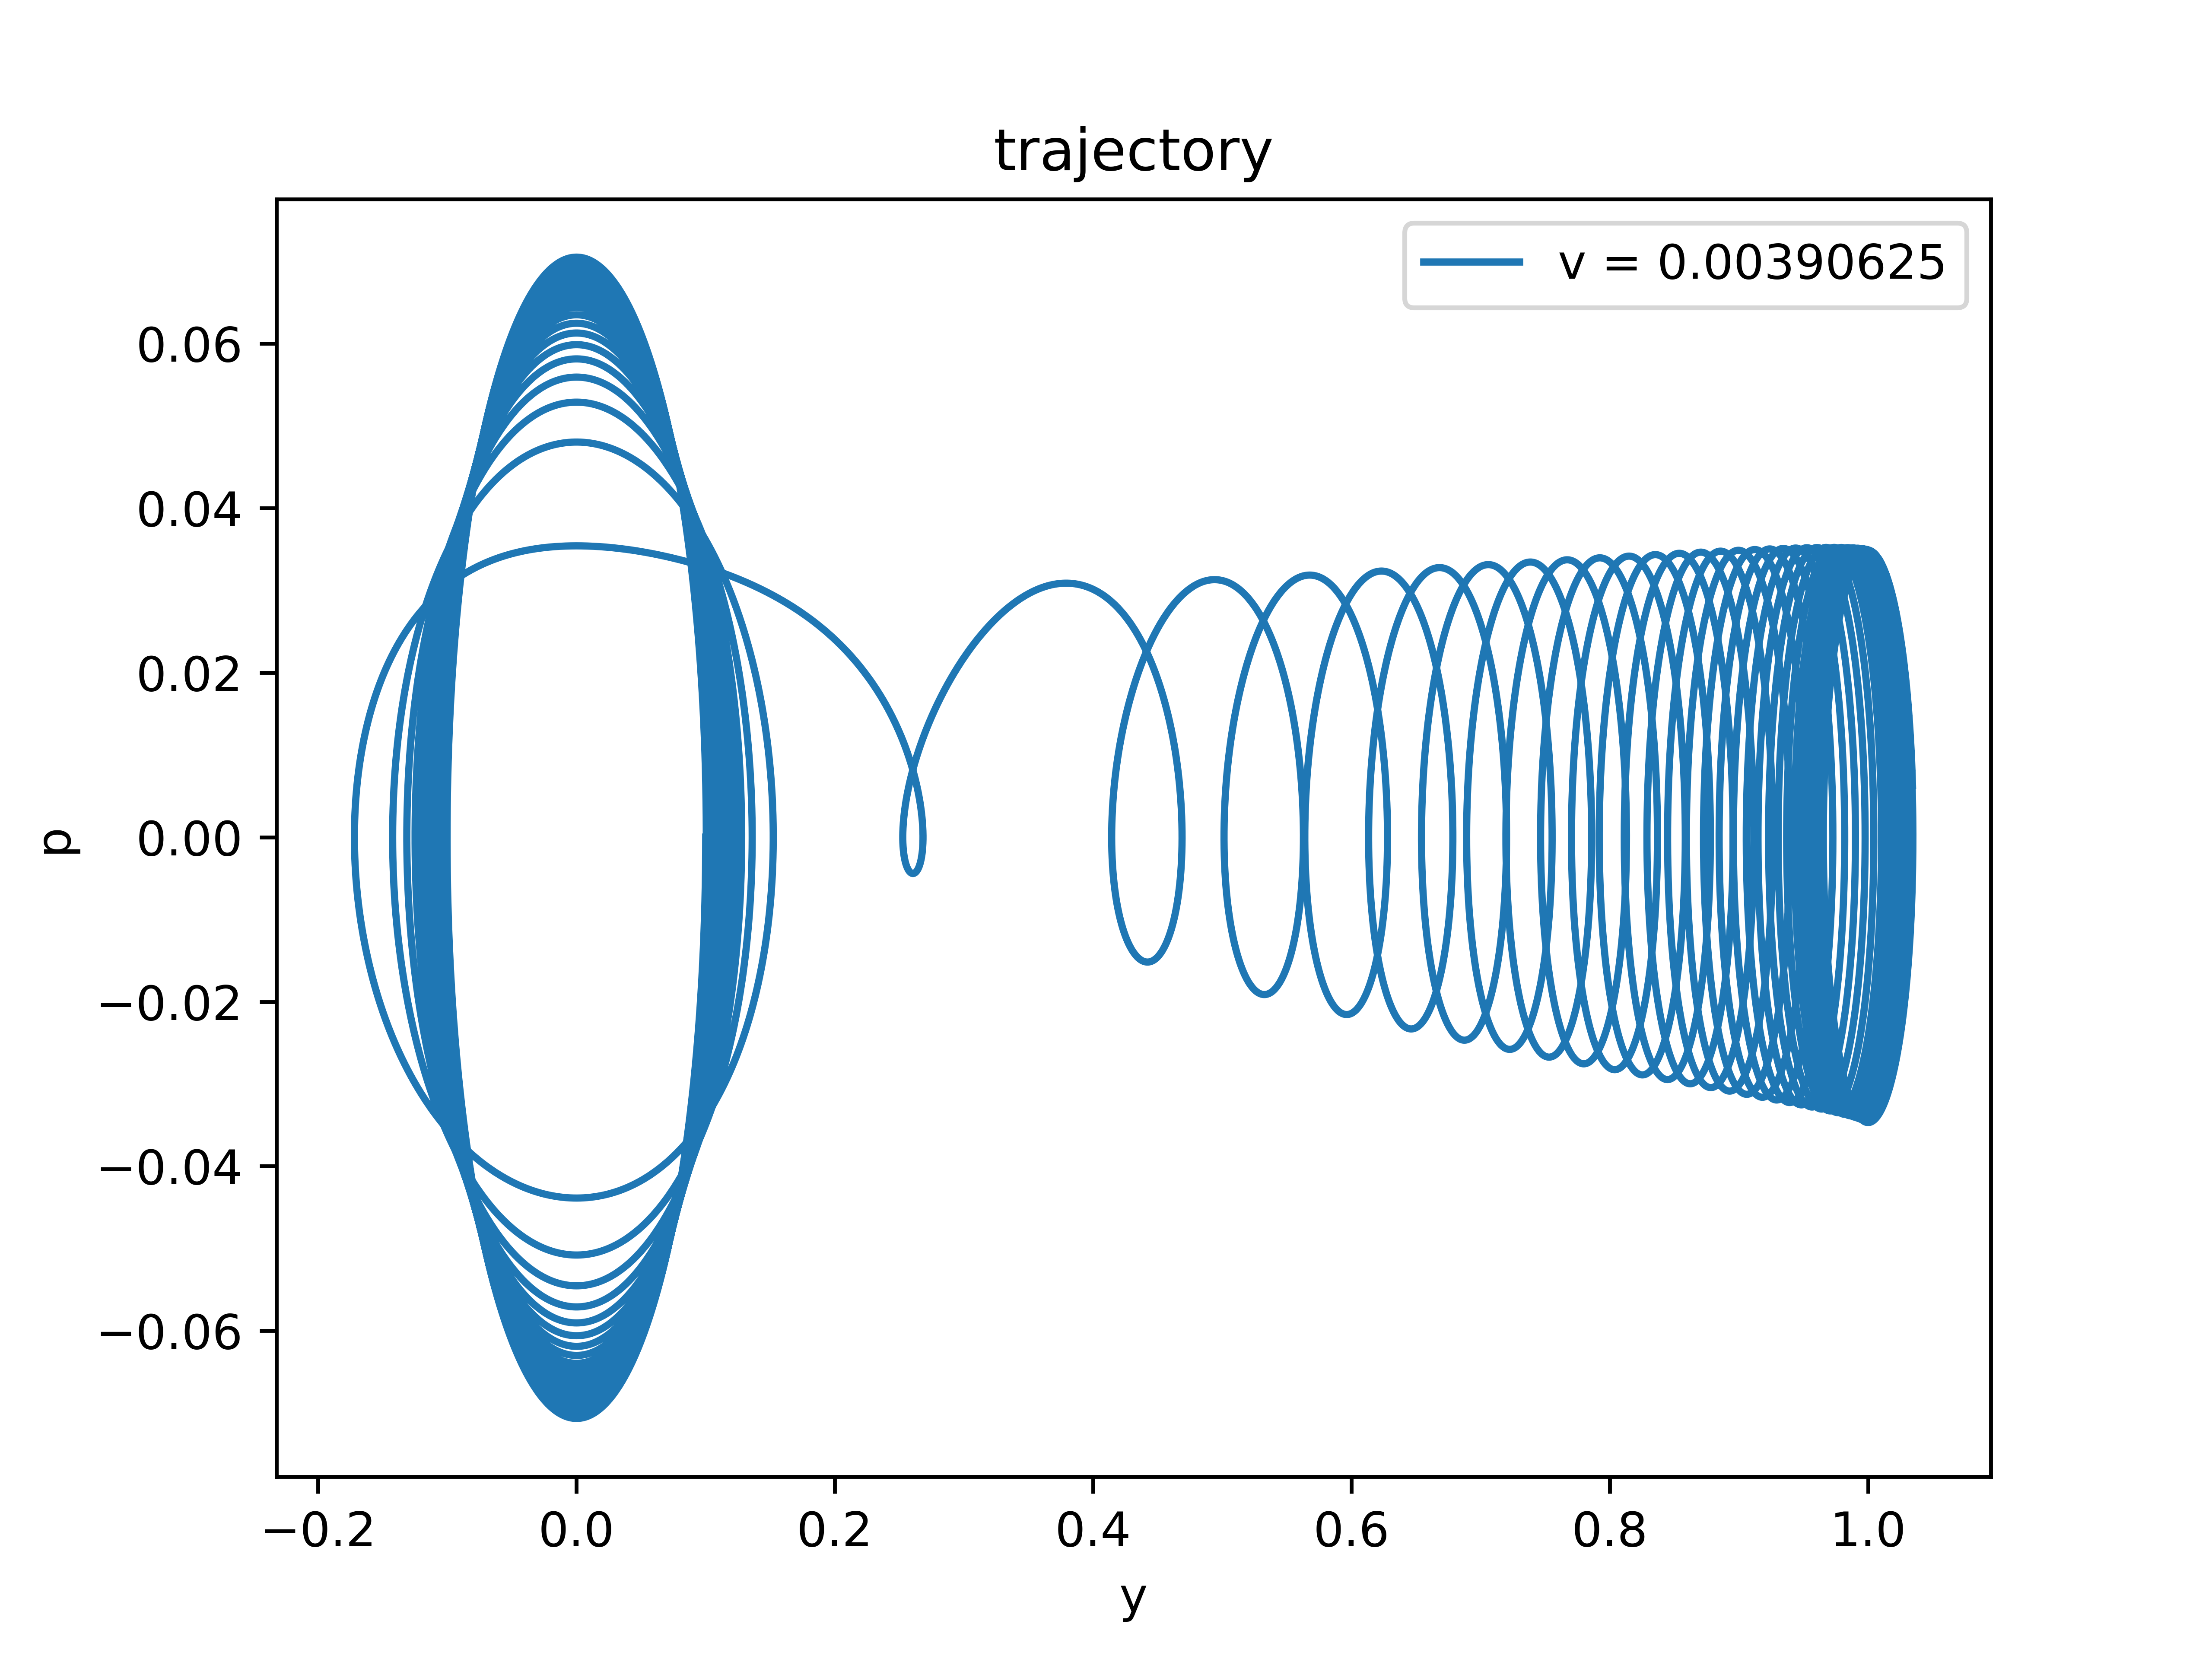
\includegraphics[scale=0.5]{2_traj_v=0_00390625.png}
        \end{tabular}
        \caption{$x$以不同速度变化时的相轨线}
        \label{v change}
    \end{table}
    \par 
    可以看到, 当参数$x$变化很快时(与系统的尺度大小近似),  运动没有在参数变化的时间范围内呈现出周期性, 当参数变化减缓时, 才能
    逐渐看到系统运动的周期性. 在参数变化的过程中, 系统会从包含一个平衡位置的状态演化到包含两个平衡位置的状态($x=1$为临界点), 
    最开始的平衡位置不再平衡, 系统的运动逐渐偏离初始值附近, 演化到新的平衡位置附近继续做稳定的运动. 所以在后面两张图中
    可以清晰地看到系统从刚开始的平衡位置逐渐演化到新平衡位置的过程, 在临界点附近展现出不规则运动. 
    \par 
    为了计算绝热不变量, 考虑将绝热不变量的积分转化为:
    \begin{equation}
        J = \frac{1}{\pi}\int_{y_{\mr{min}}}^{y_{\mr{max}}}\sqrt{\frac{2(E - V(y))}{(y - y_{\mr{min}})(y_{\mr{max}} - y)}}
        \sqrt{(y - y_{\mr{min}})(y_{\mr{max}} - y)} \d y
    \end{equation}
    考虑使用数值求根的方法求出对应的函数零点, 具体在程序中采用Dekker法求根. 但是涉及到根有多个的情况, 
    为了求出我们想要的根, 需要进一步分析问题的性质. 可以想象系统在一个变化的势场中运动, 这个势场从单势阱
    变化到双势阱, 因此首先判断势能中心与总能量的关系, 如果势能中心小于总能量, 那么系统可以穿透势垒, 直接在
    $y>0,y<0$的地方分别求根; 否则, 由于问题的对称性, 可以选择在$y>0$的部分讨论, 首先求出势能函数的极值点,
    以极值点为分界分别求根, 当求出两个根后, 考虑直接使用Chebyshev第二类积分计算绝热不变量:
    \begin{lstlisting}
        E = energy(y[0], p[0]);
        if (E - potential(0.0) > 0) {
          y_min = dekker_root(tunnel_points, -2, 0, 1e-5);
          y_max = dekker_root(tunnel_points, 0, 2, 1e-5);
        } // only two tunnelling points
        else {
          double y_M = 0; // find the minimium of V to determine the root
          y_M = golden_section_opt(potential_inverse, 0, 2, 1e-5);
          y_min = dekker_root(tunnel_points, 0, y_M, 1e-5);
          y_max = dekker_root(tunnel_points, y_M, 2, 1e-5);
        }
        J = chebyshev_second_integral(J_func, y_min, y_max, 1e2);
    \end{lstlisting}
    Dekker法求根和求极值使用的黄金分割-抛物线相结合的方法见1\_D\_optimize.cpp,
     Chebyshev积分见integral.cpp. 注意到在计算Chebyshev积分时选区的格点并不多, 有两个原因: 
     首先此数值方法精度较高, 选取过多的点有点浪费; 其次当选取点太密时容易在被积函数中出现0/0,
     会导致个别点积分值数值发散, 仔细观察了发散点周围的数值, 均比较连续, 因此认为这种发散是由于数值精度
     造成的, 故应该设法避免.
     \par 
     将绝热不变量随外参数的变化绘制于表\ref{v change J}中:
     \begin{table}[htbp]
        \centering
        \begin{tabular}[htbp]{cc}
            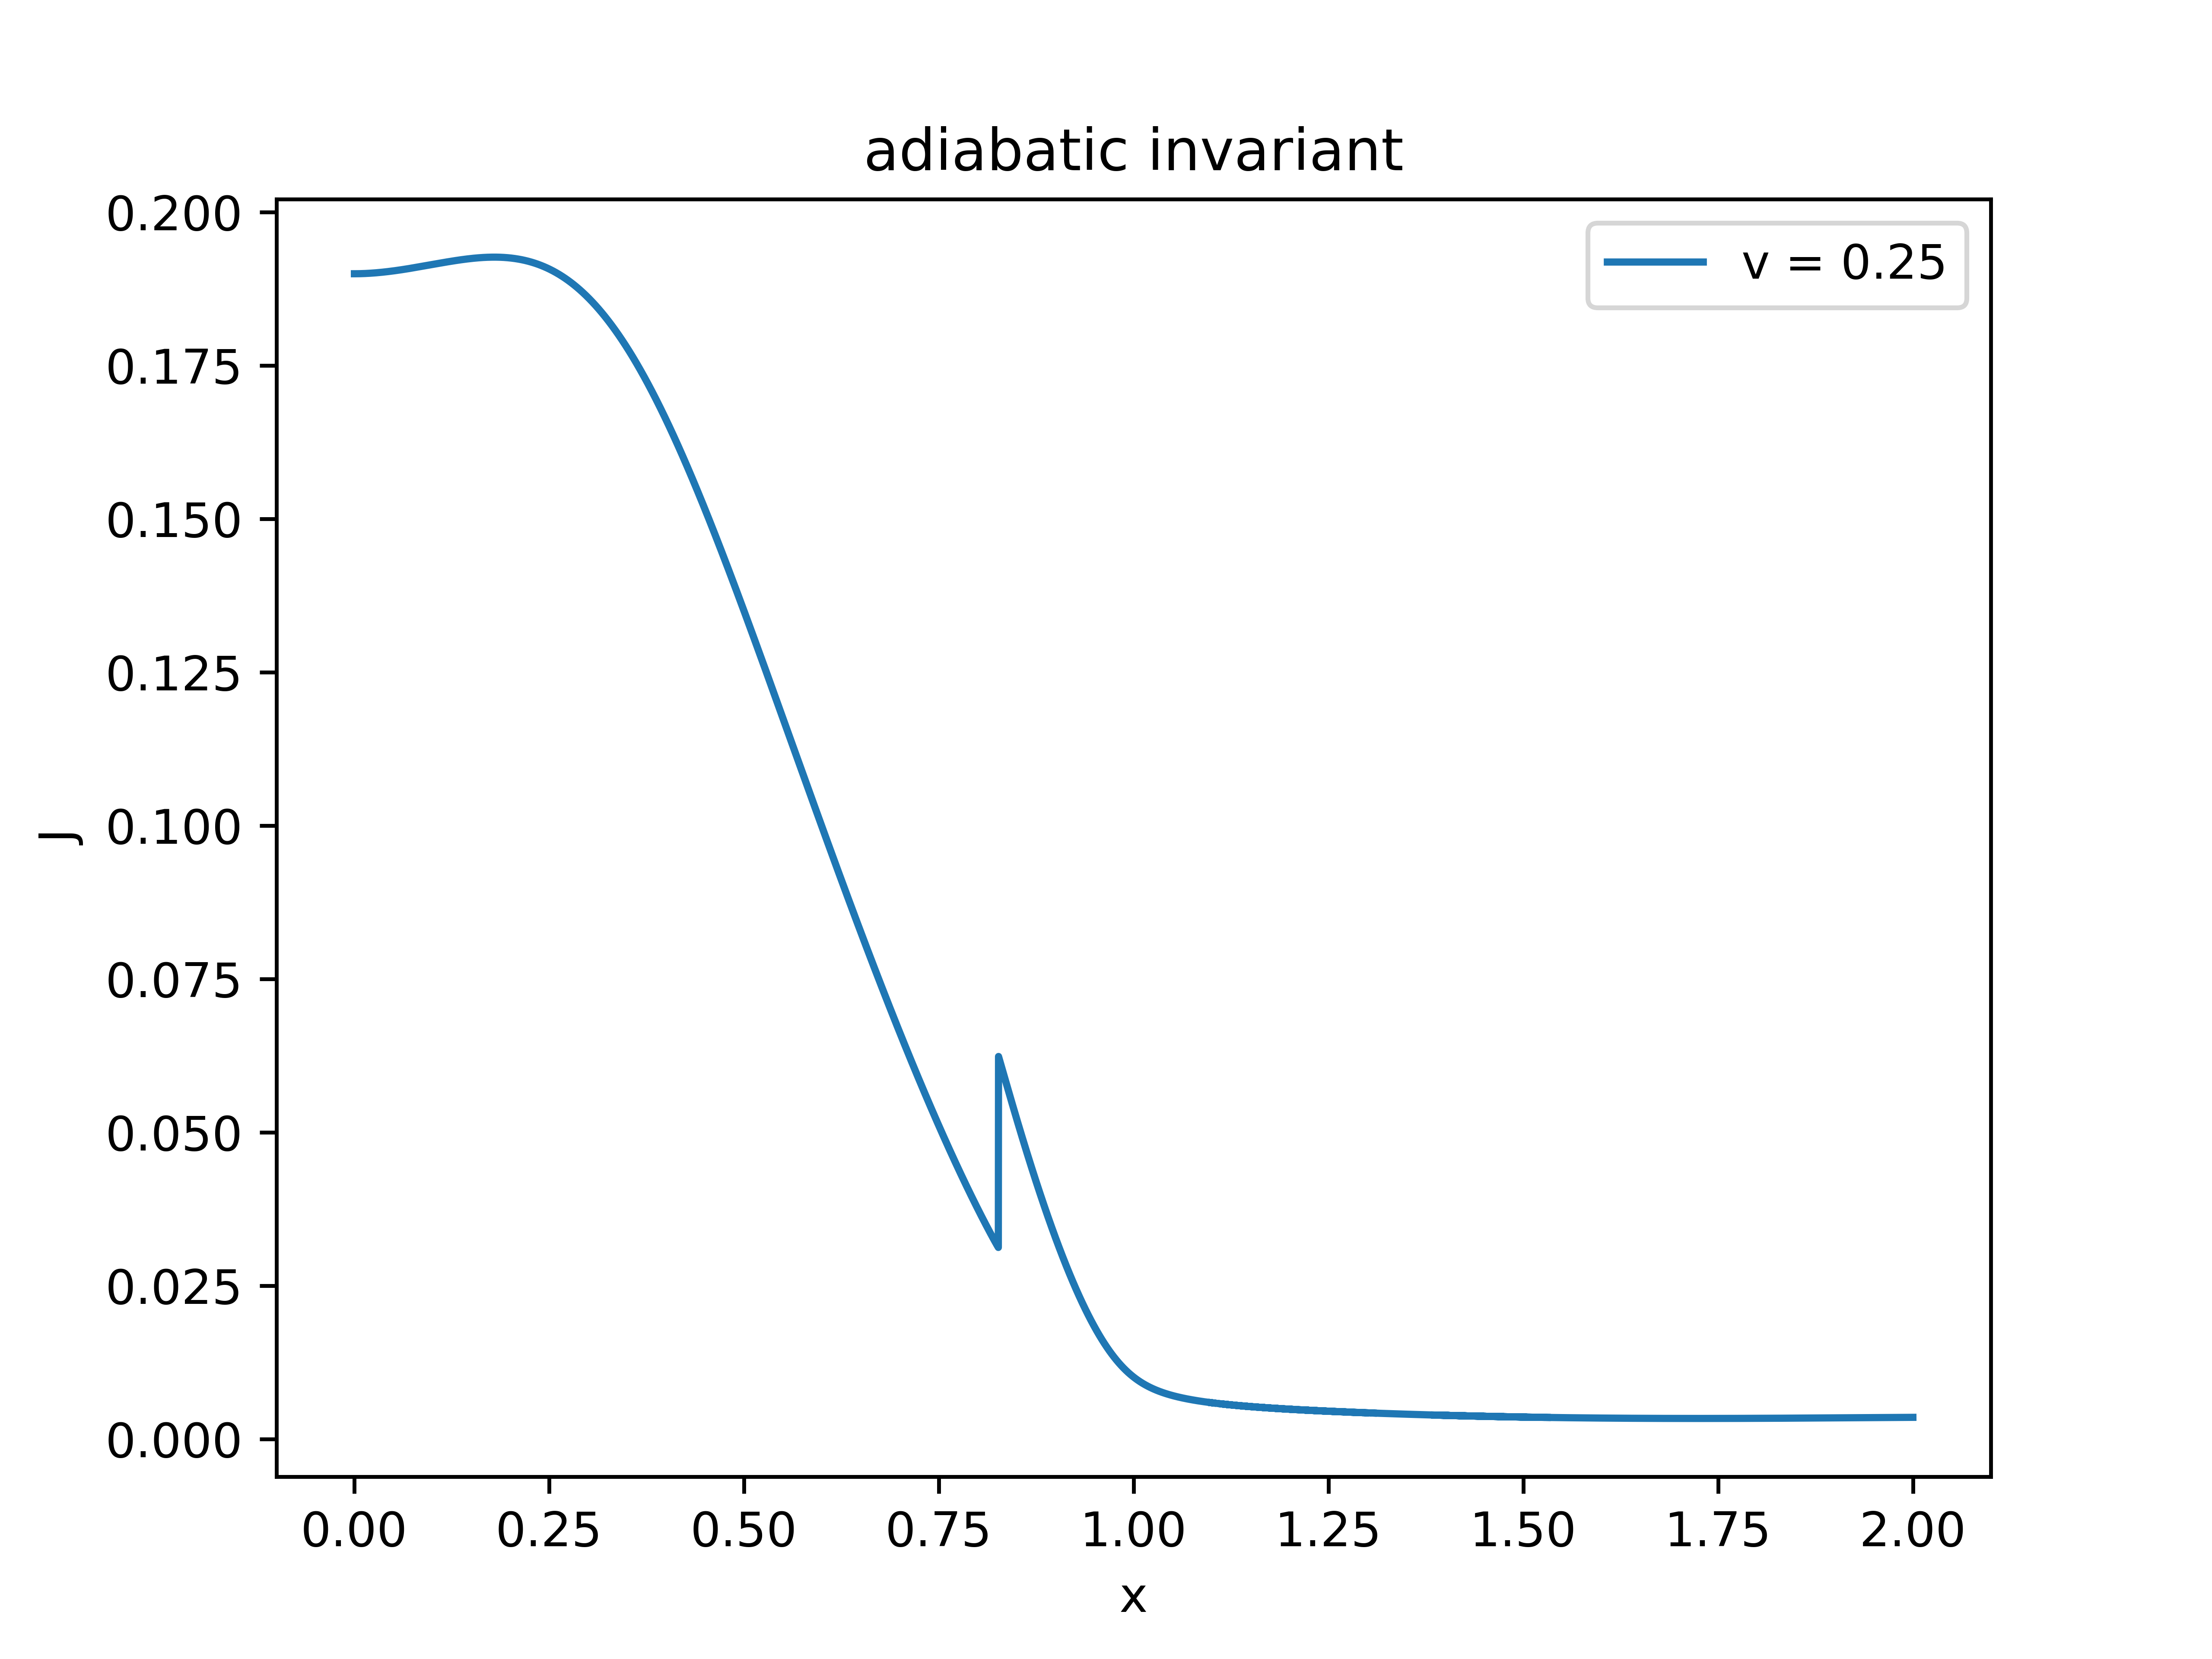
\includegraphics[scale=0.5]{2_ad_invr_v=0_25.png} & 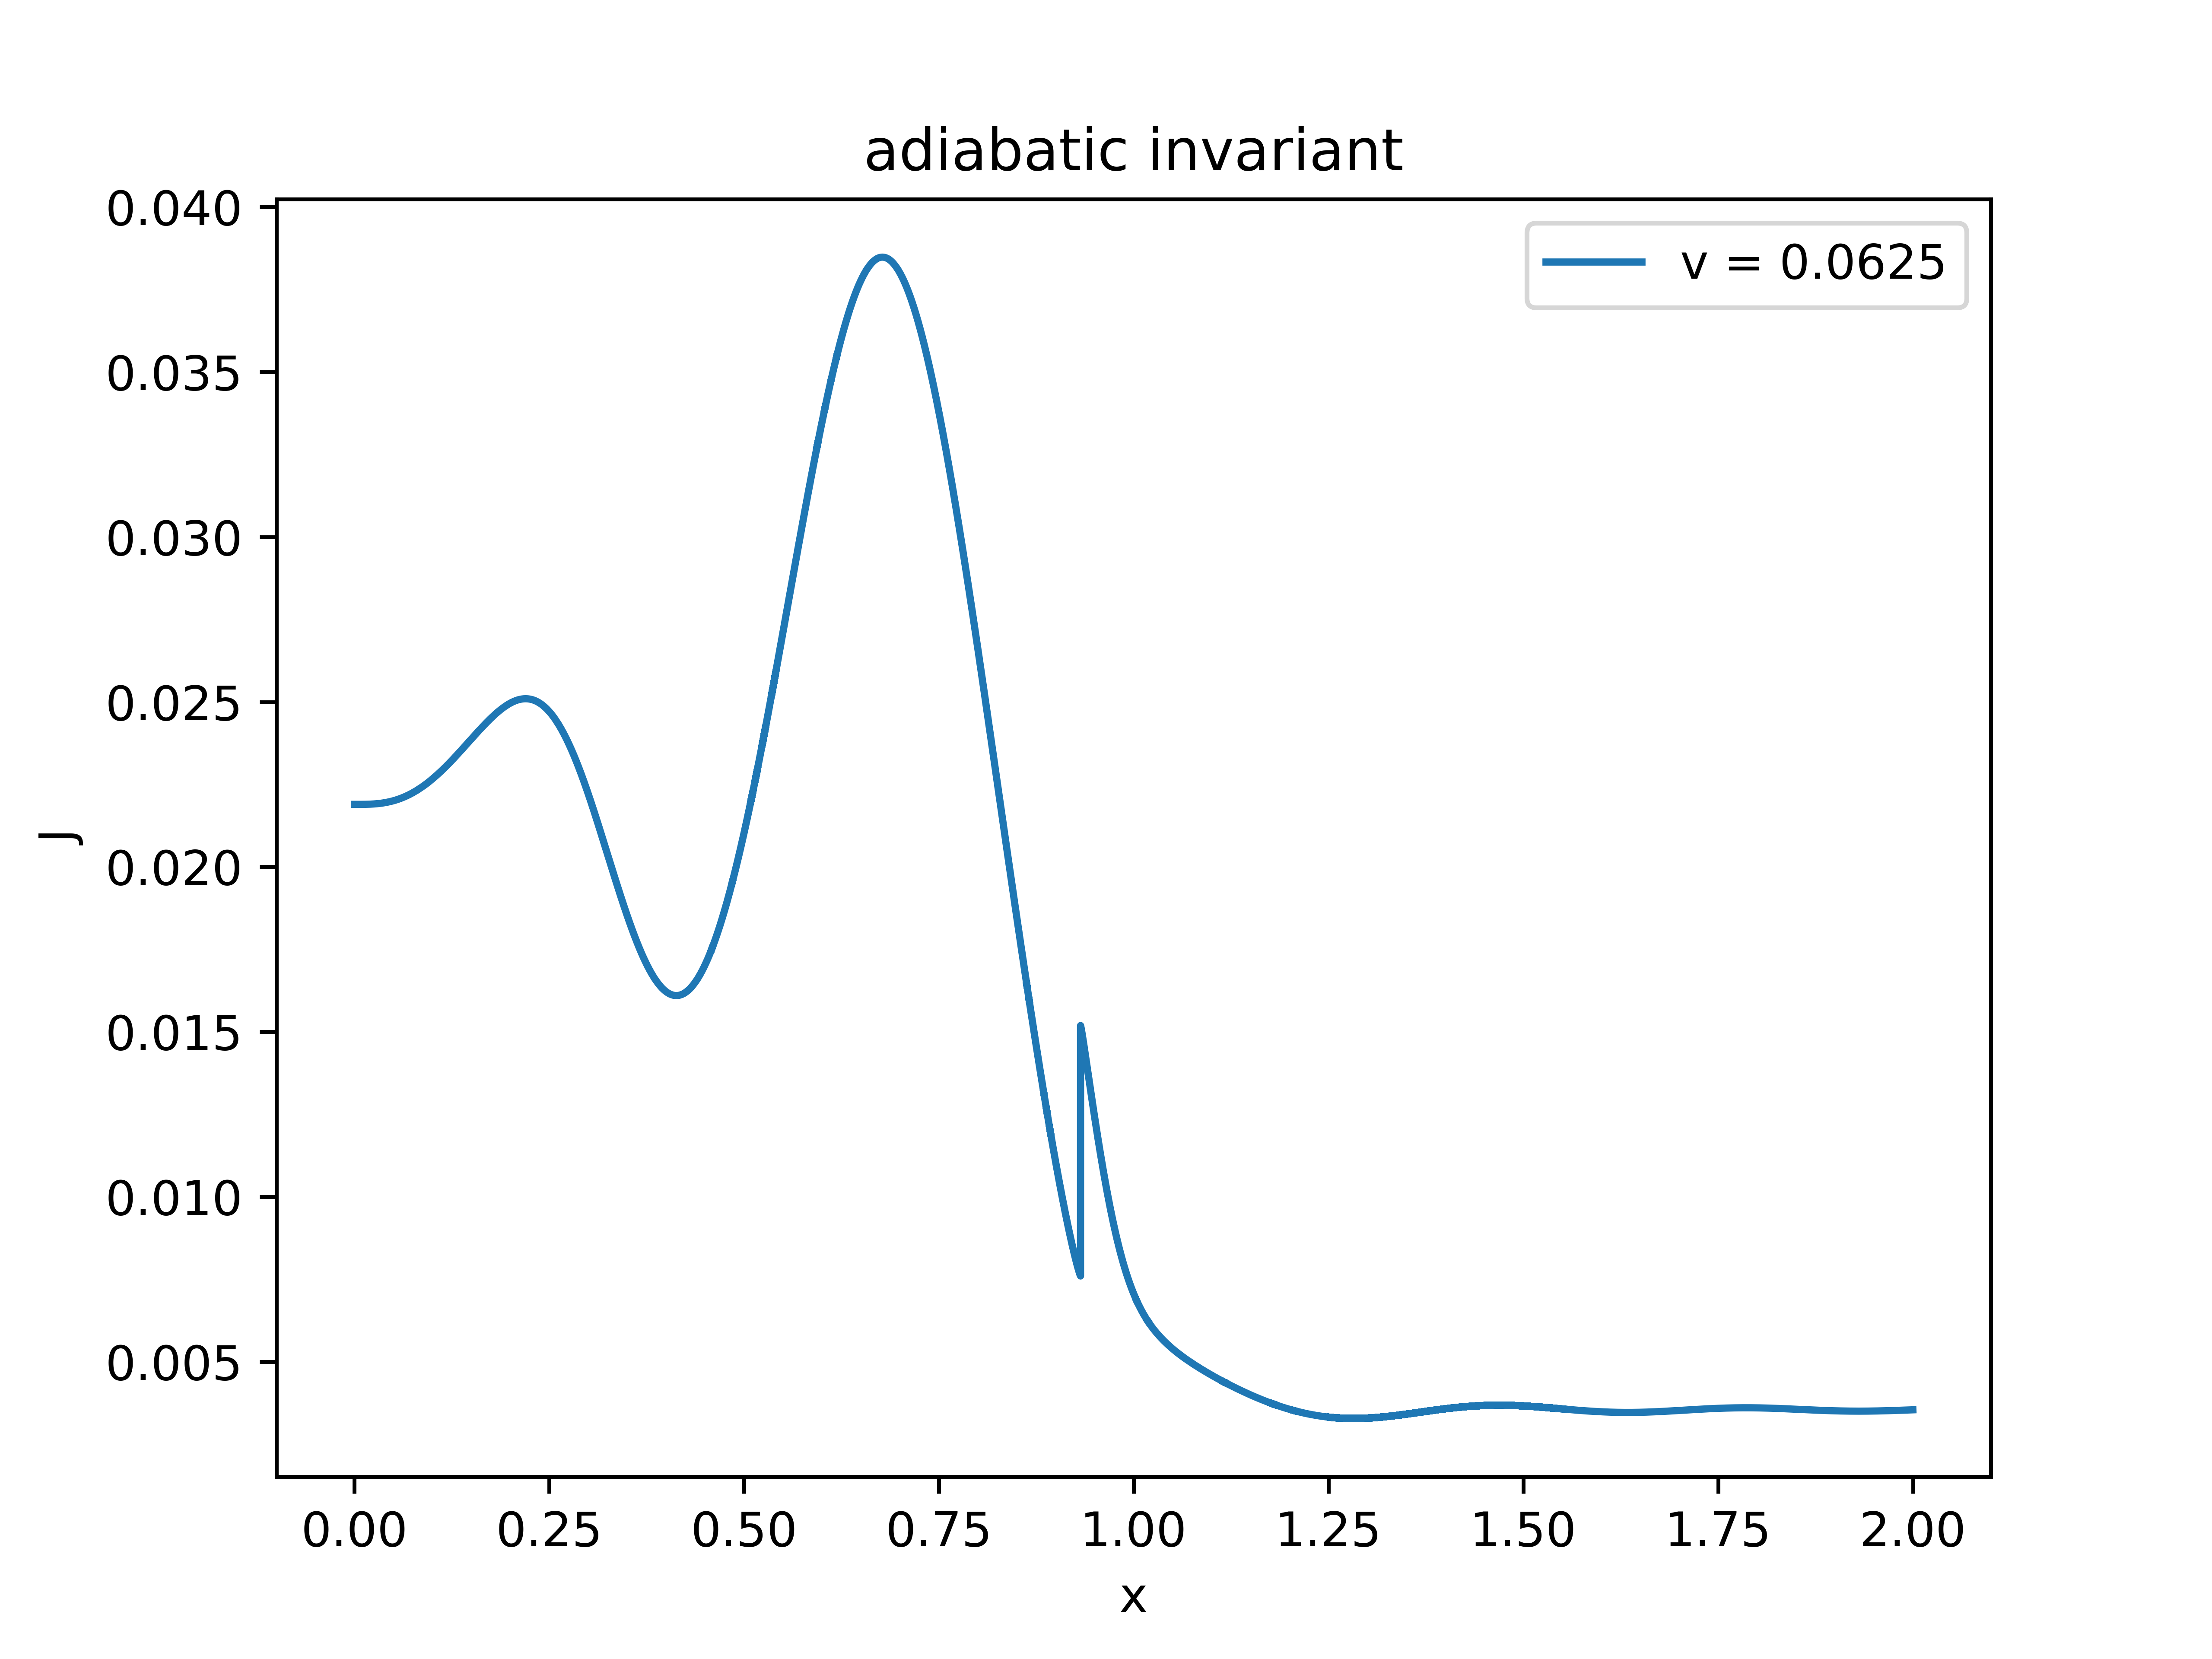
\includegraphics[scale=0.5]{2_ad_invr_v=0_0625.png} \\
            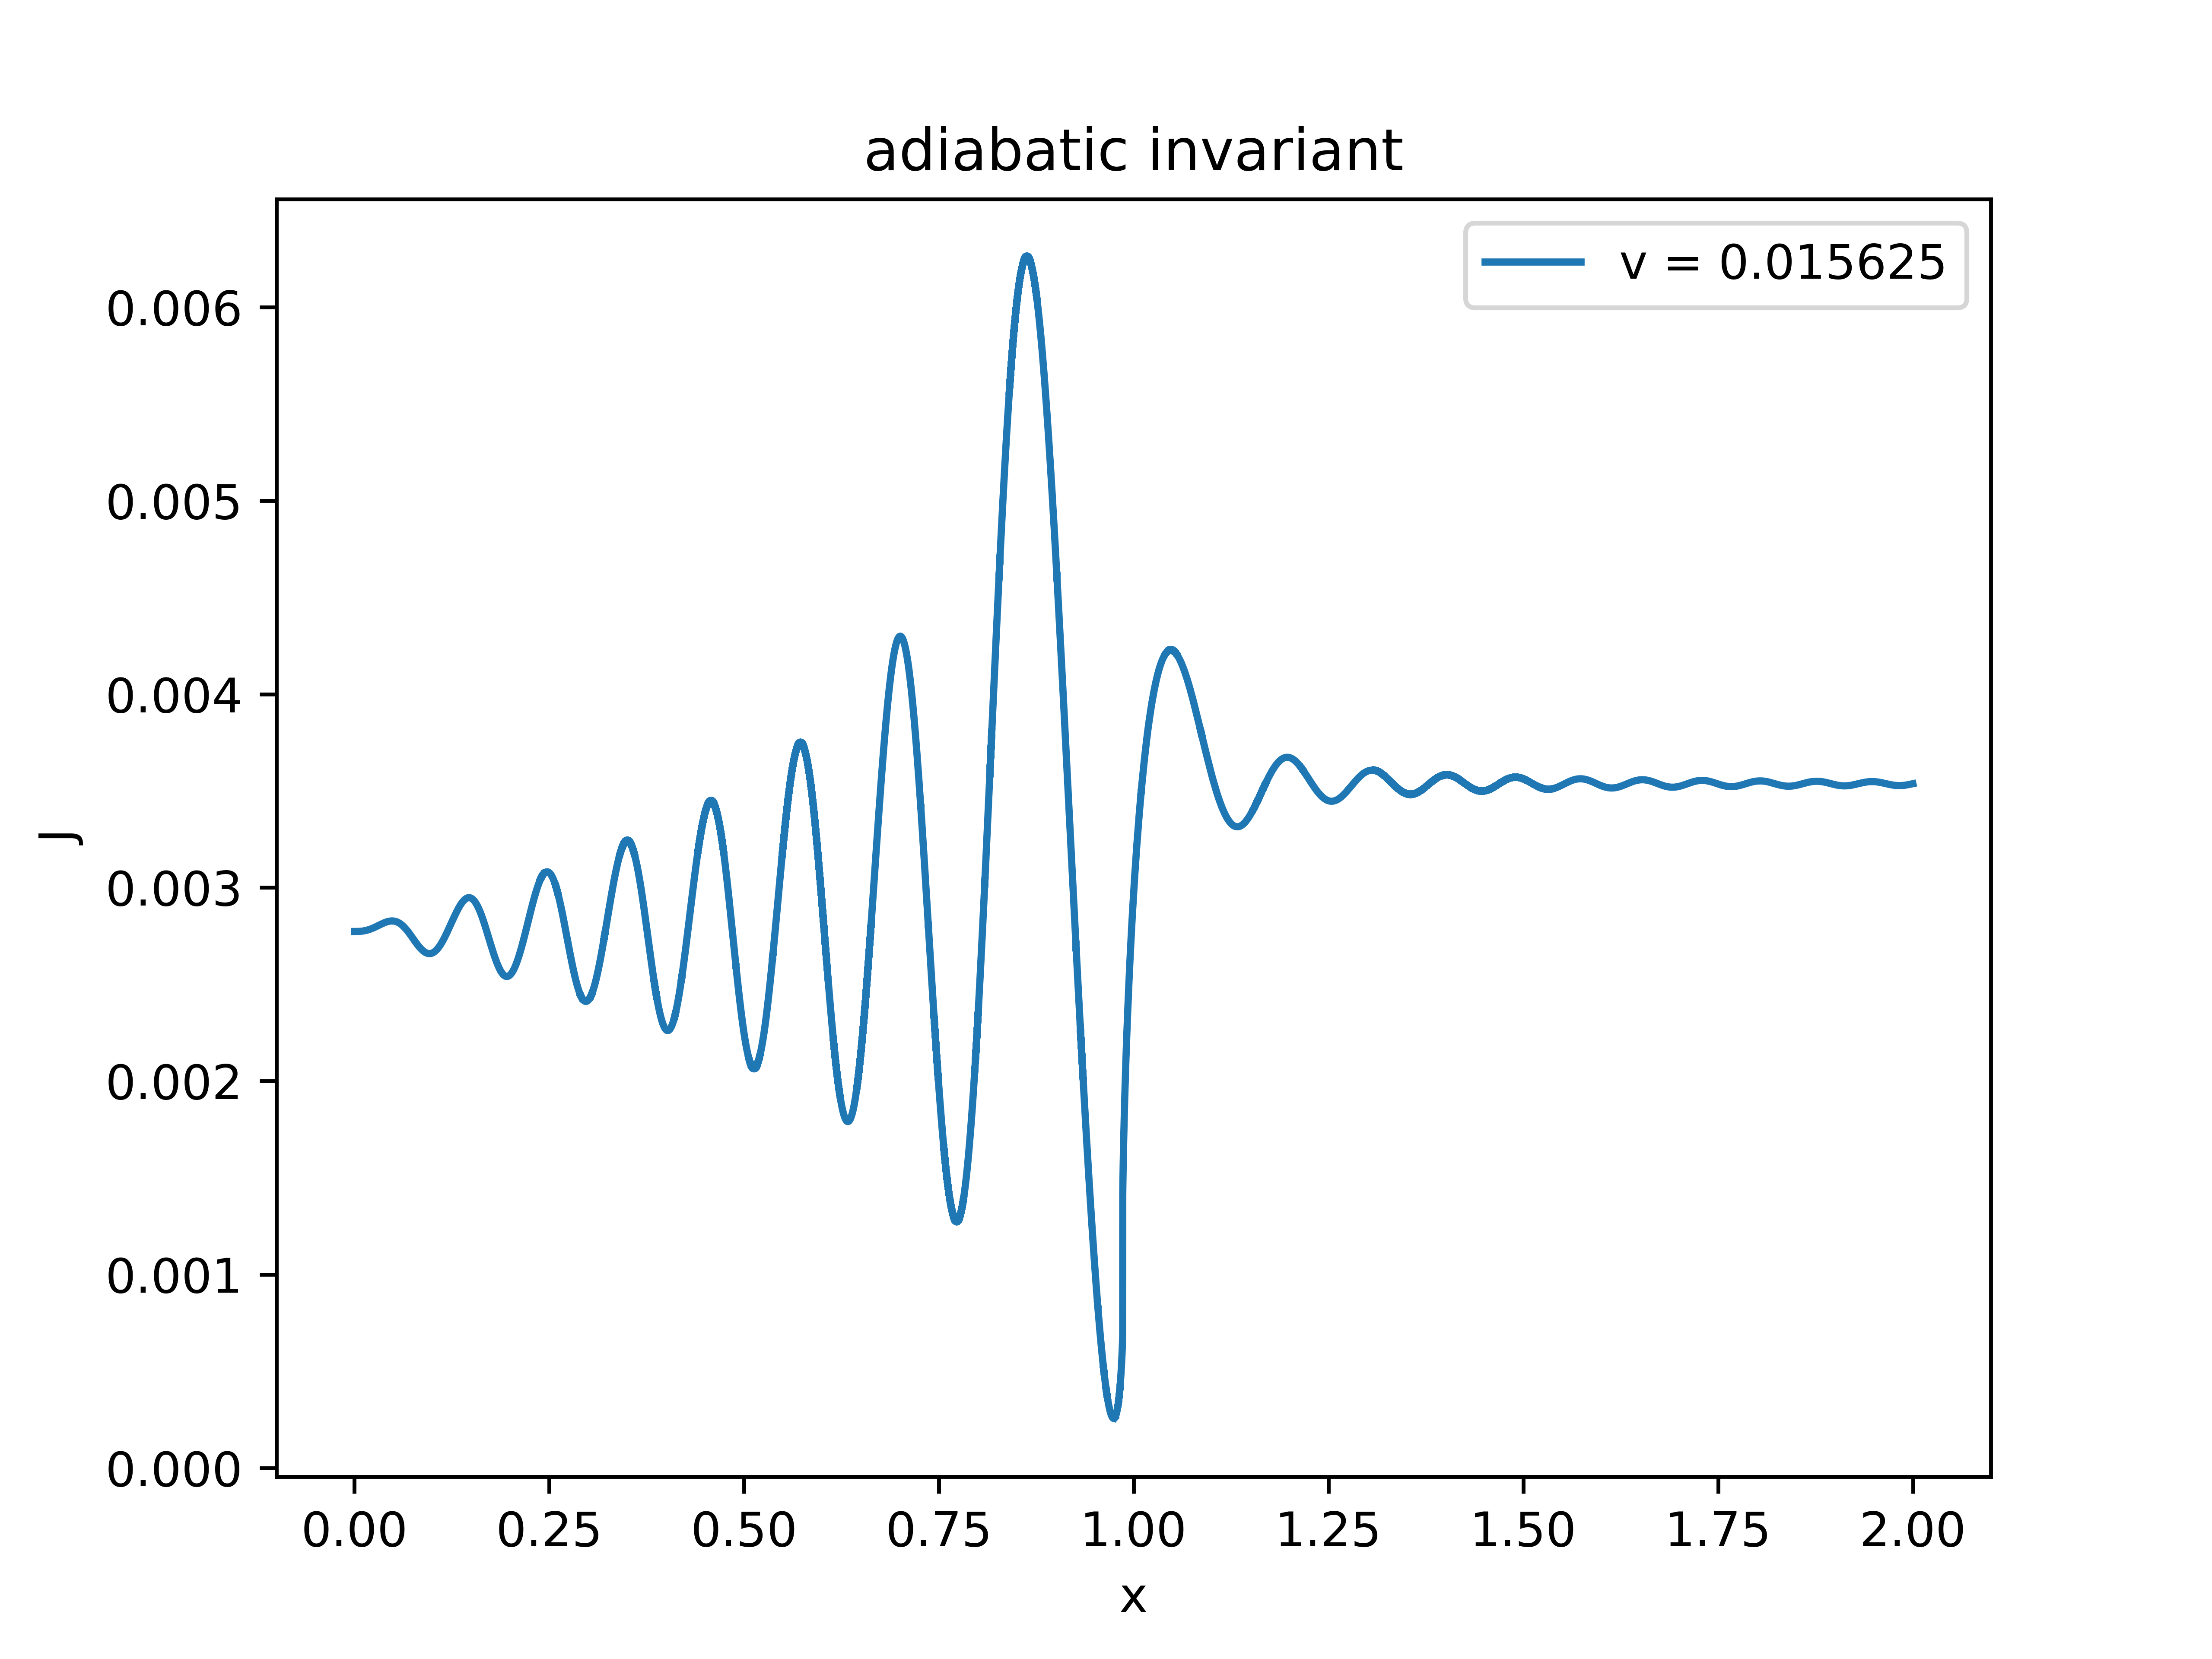
\includegraphics[scale=0.5]{2_ad_invr_v=0_015625.png} & 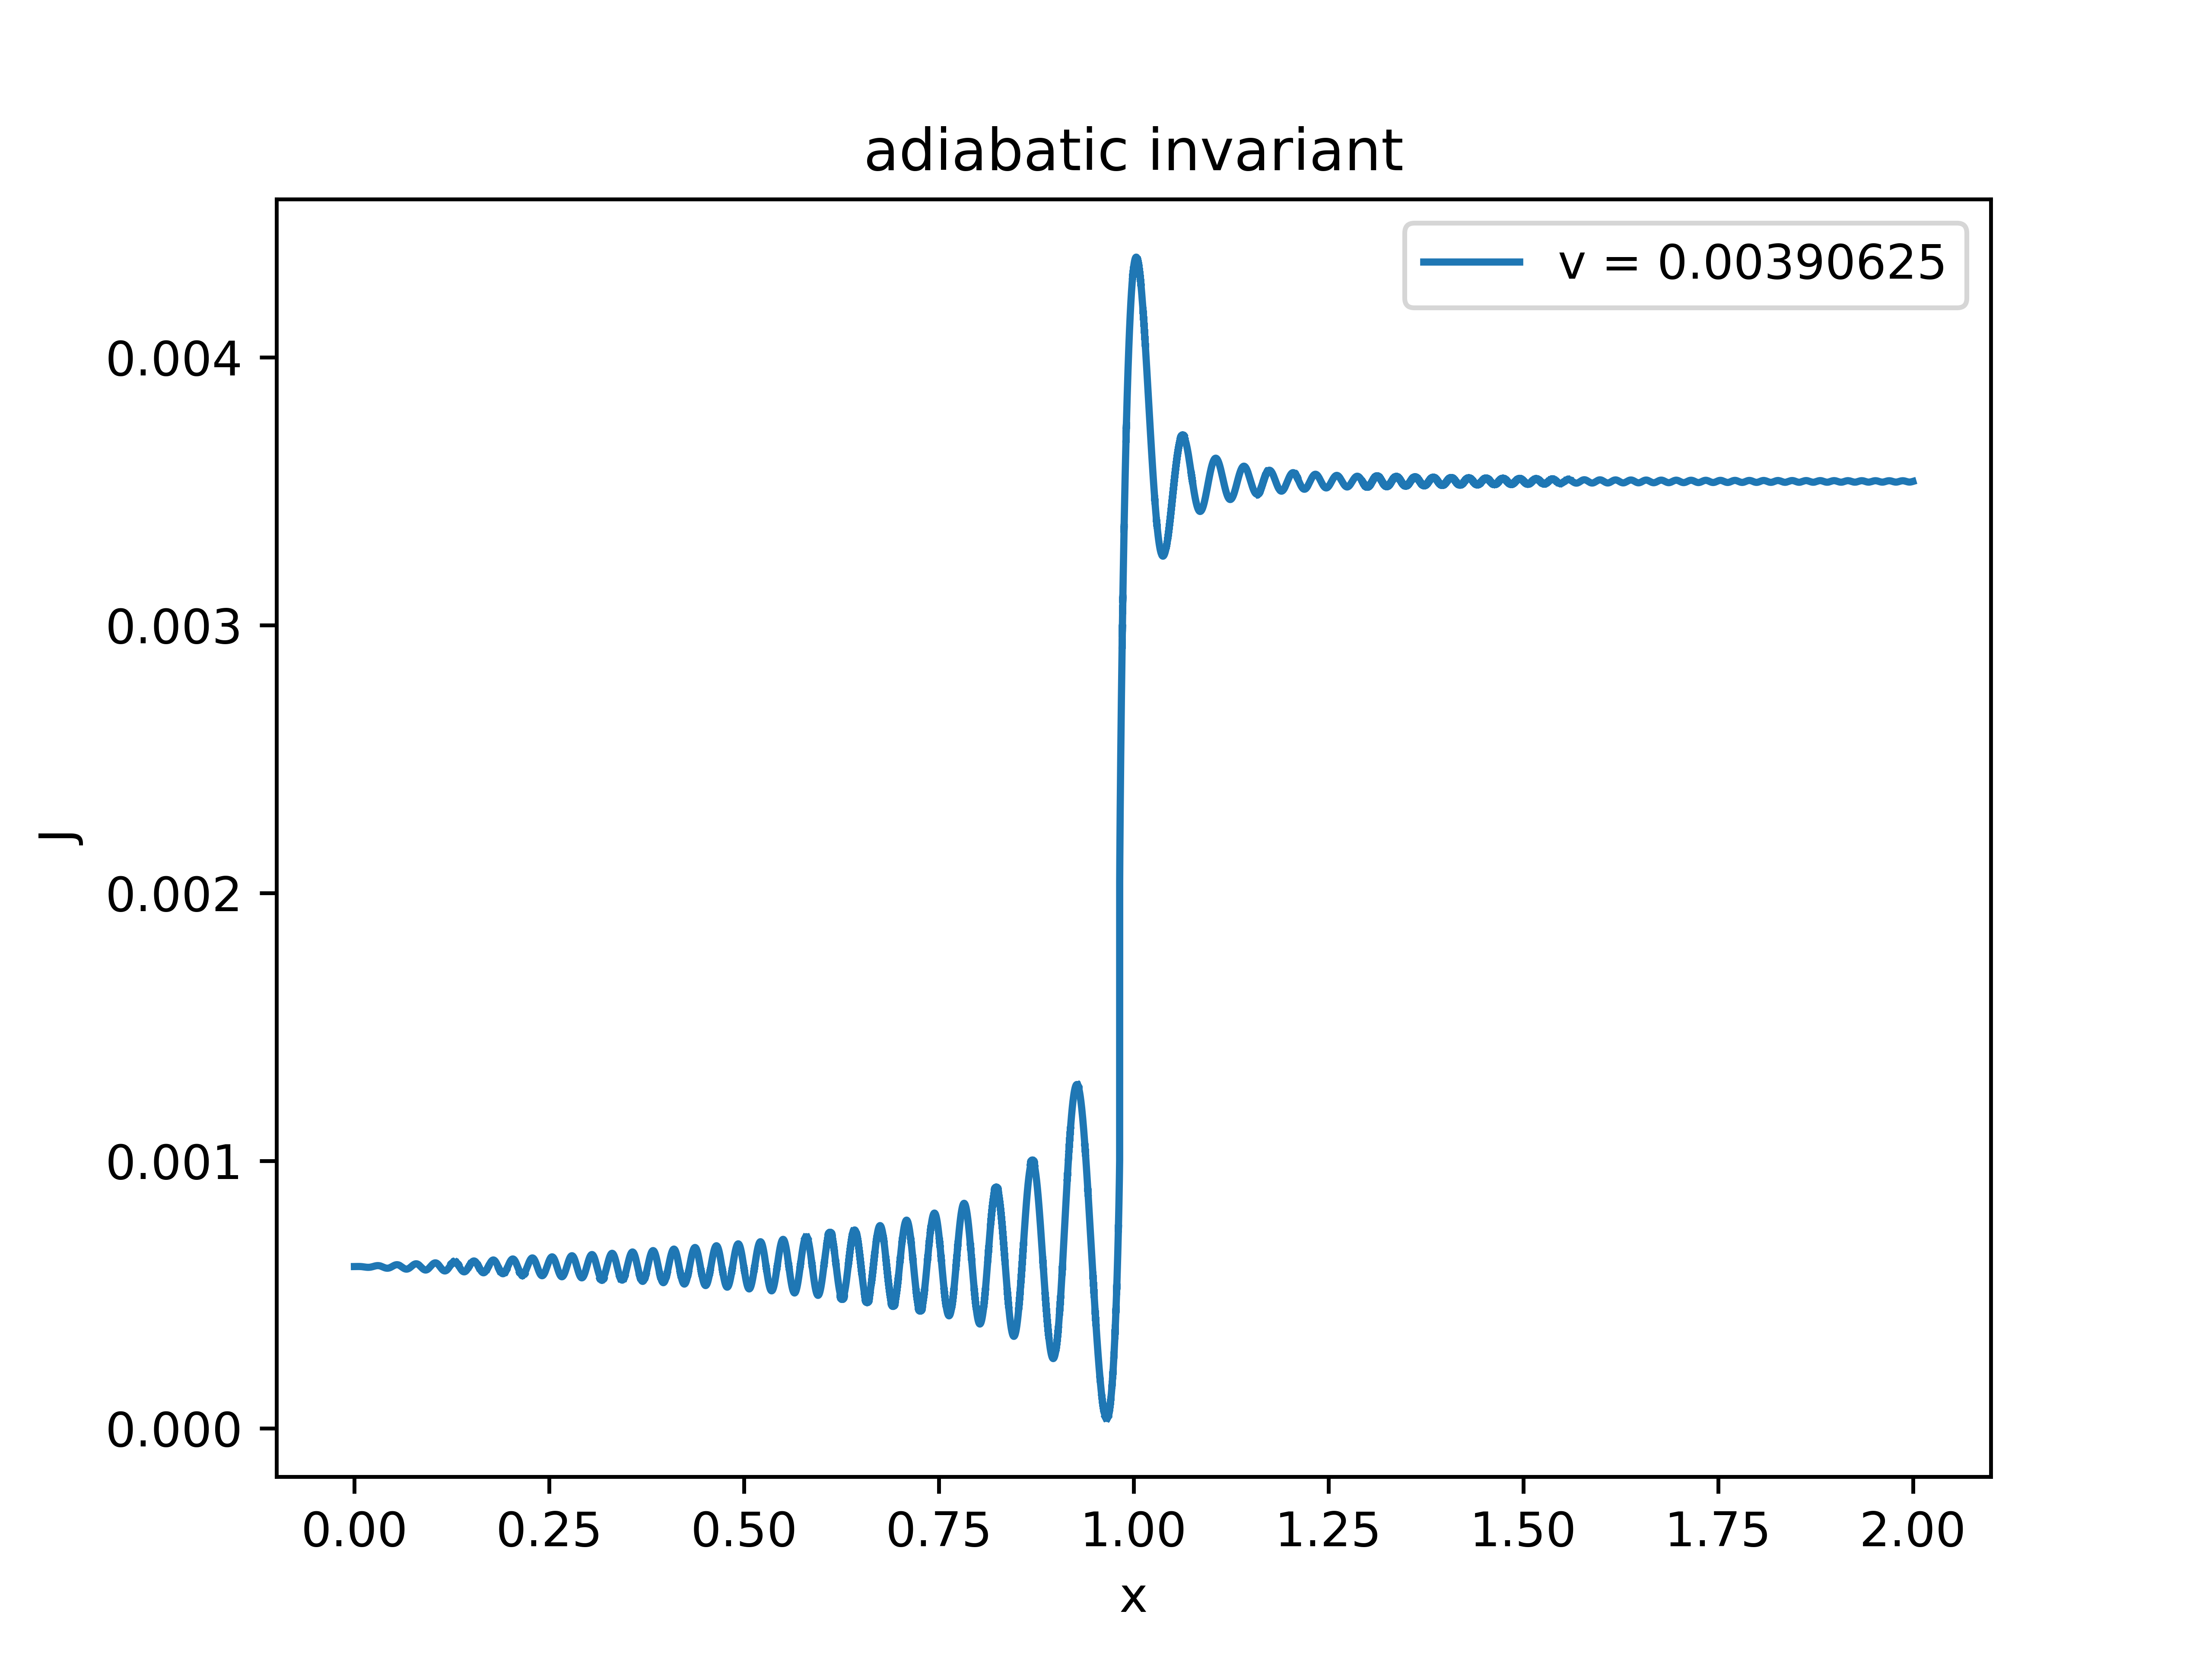
\includegraphics[scale=0.5]{2_ad_invr_v=0_00390625.png}
        \end{tabular}
        \caption{$x$以不同速度变化时的绝热不变量$J$的变化}
        \label{v change J}
    \end{table}
    可以看到, 当外参数随时间缓慢变化时, 系统的绝热不变量确实基本保持稳定, 但是如果系统的运动接近于或者将要跨越
    不稳定平衡点, 绝热不变量会快速震荡. 得出结论, 只要外参数改变的过程中系统的平衡位置的性质(个数及稳定性)
    不发生改变, 绝热定理是普适的; 或者说绝热定理在外参数变化的某个邻域内总局部成立.

    \subsubsection{$g$作为缓变参数}
    使用Velocity-Verlet方法容易计算出$g$变化半个周期之内系统的相轨迹, 结果列于表\ref{g change}中:
    \begin{table}[htbp]
        \centering
        \begin{tabular}[htbp]{cc}
            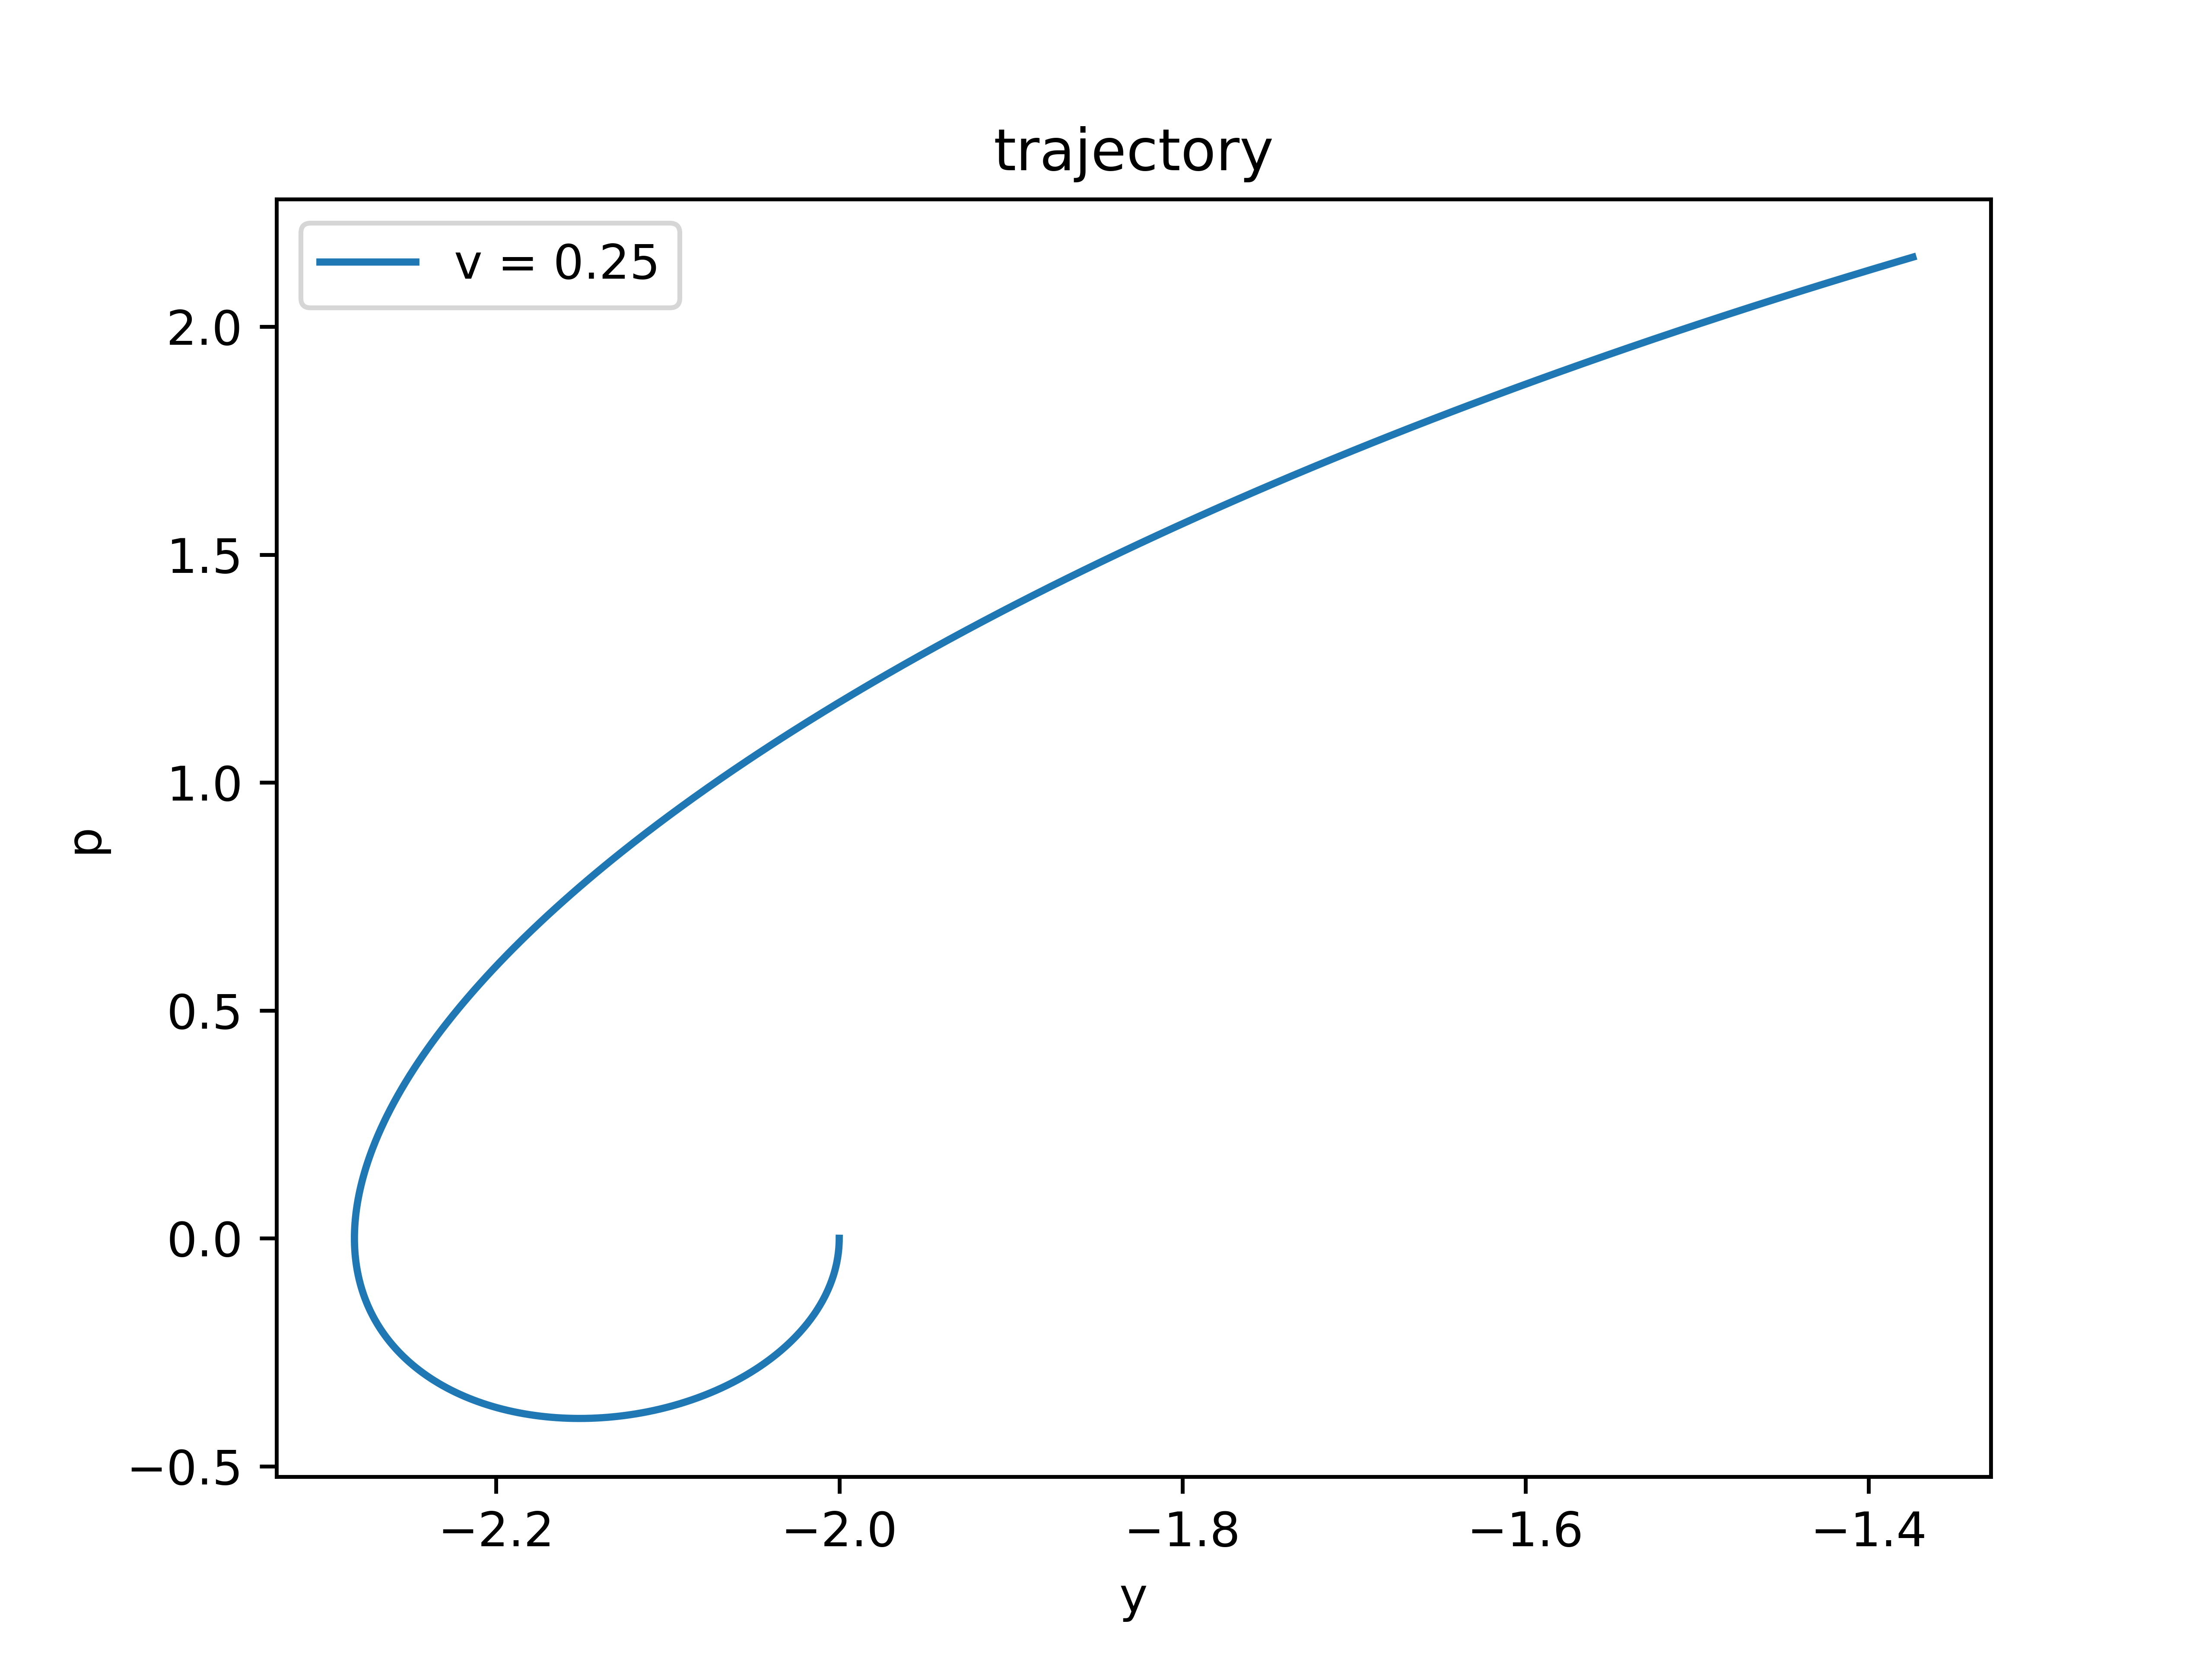
\includegraphics[scale=0.5]{3_traj_v=0_25.png} & 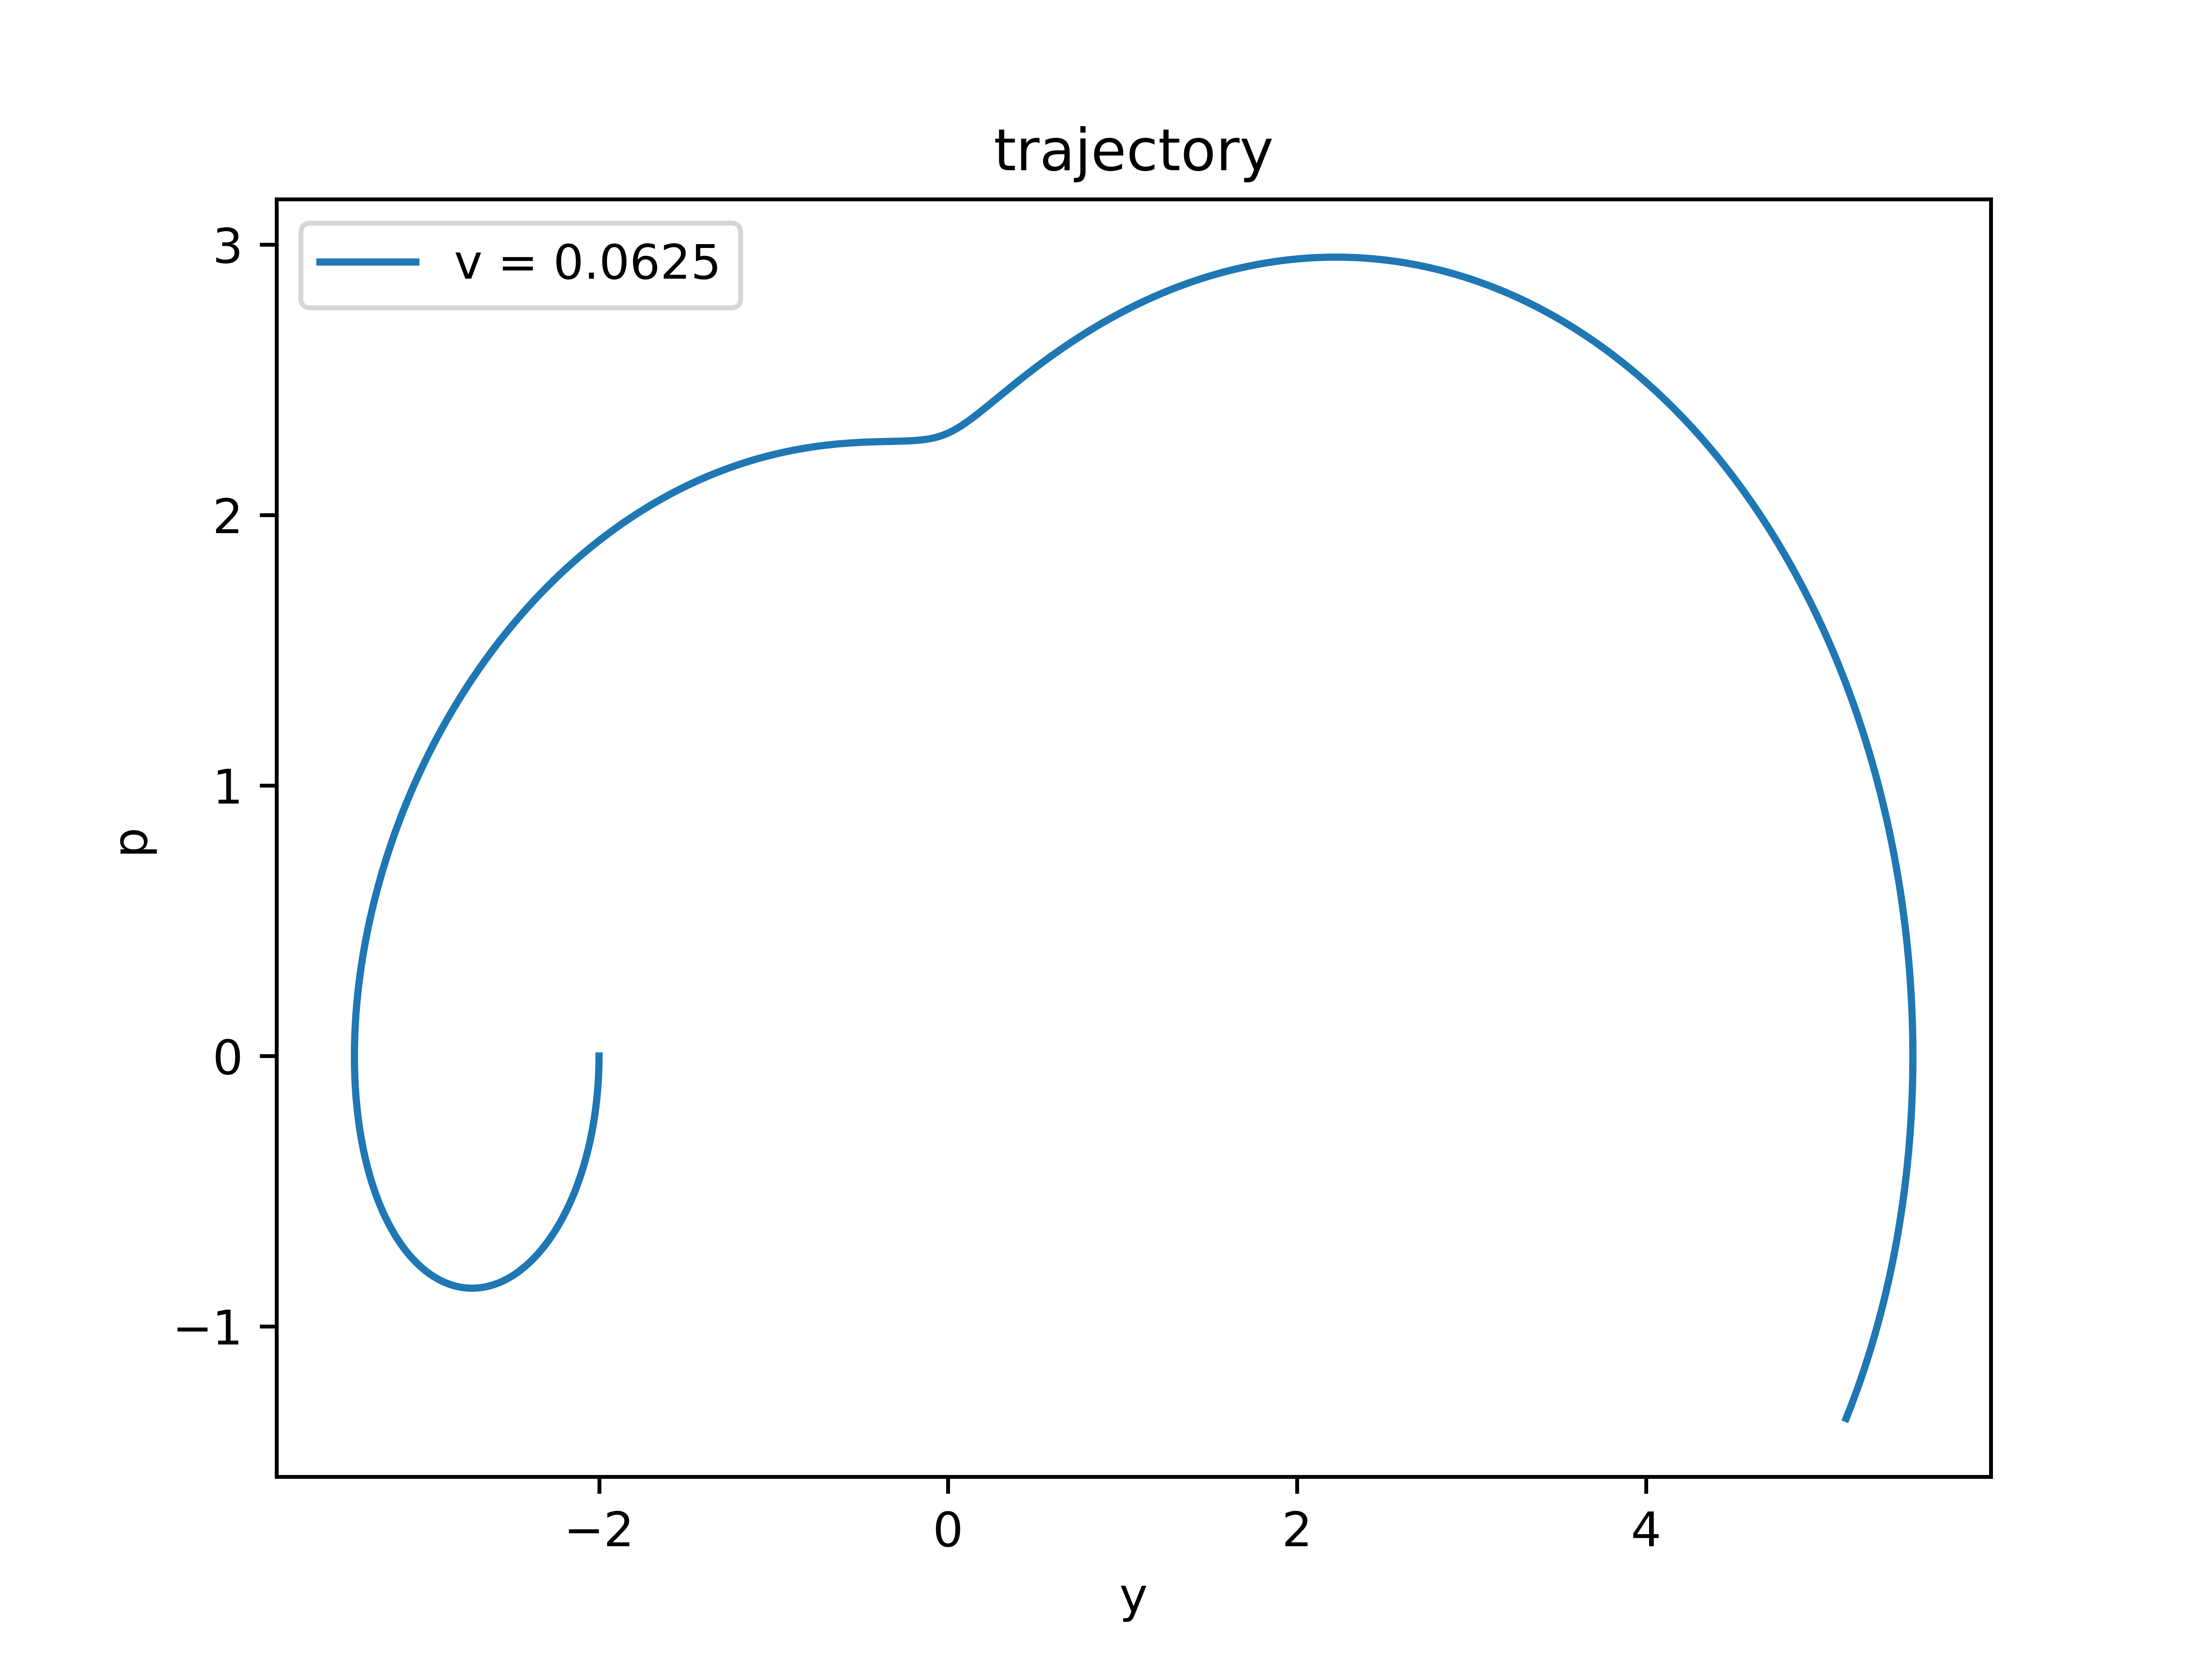
\includegraphics[scale=0.5]{3_traj_v=0_0625.png} \\
            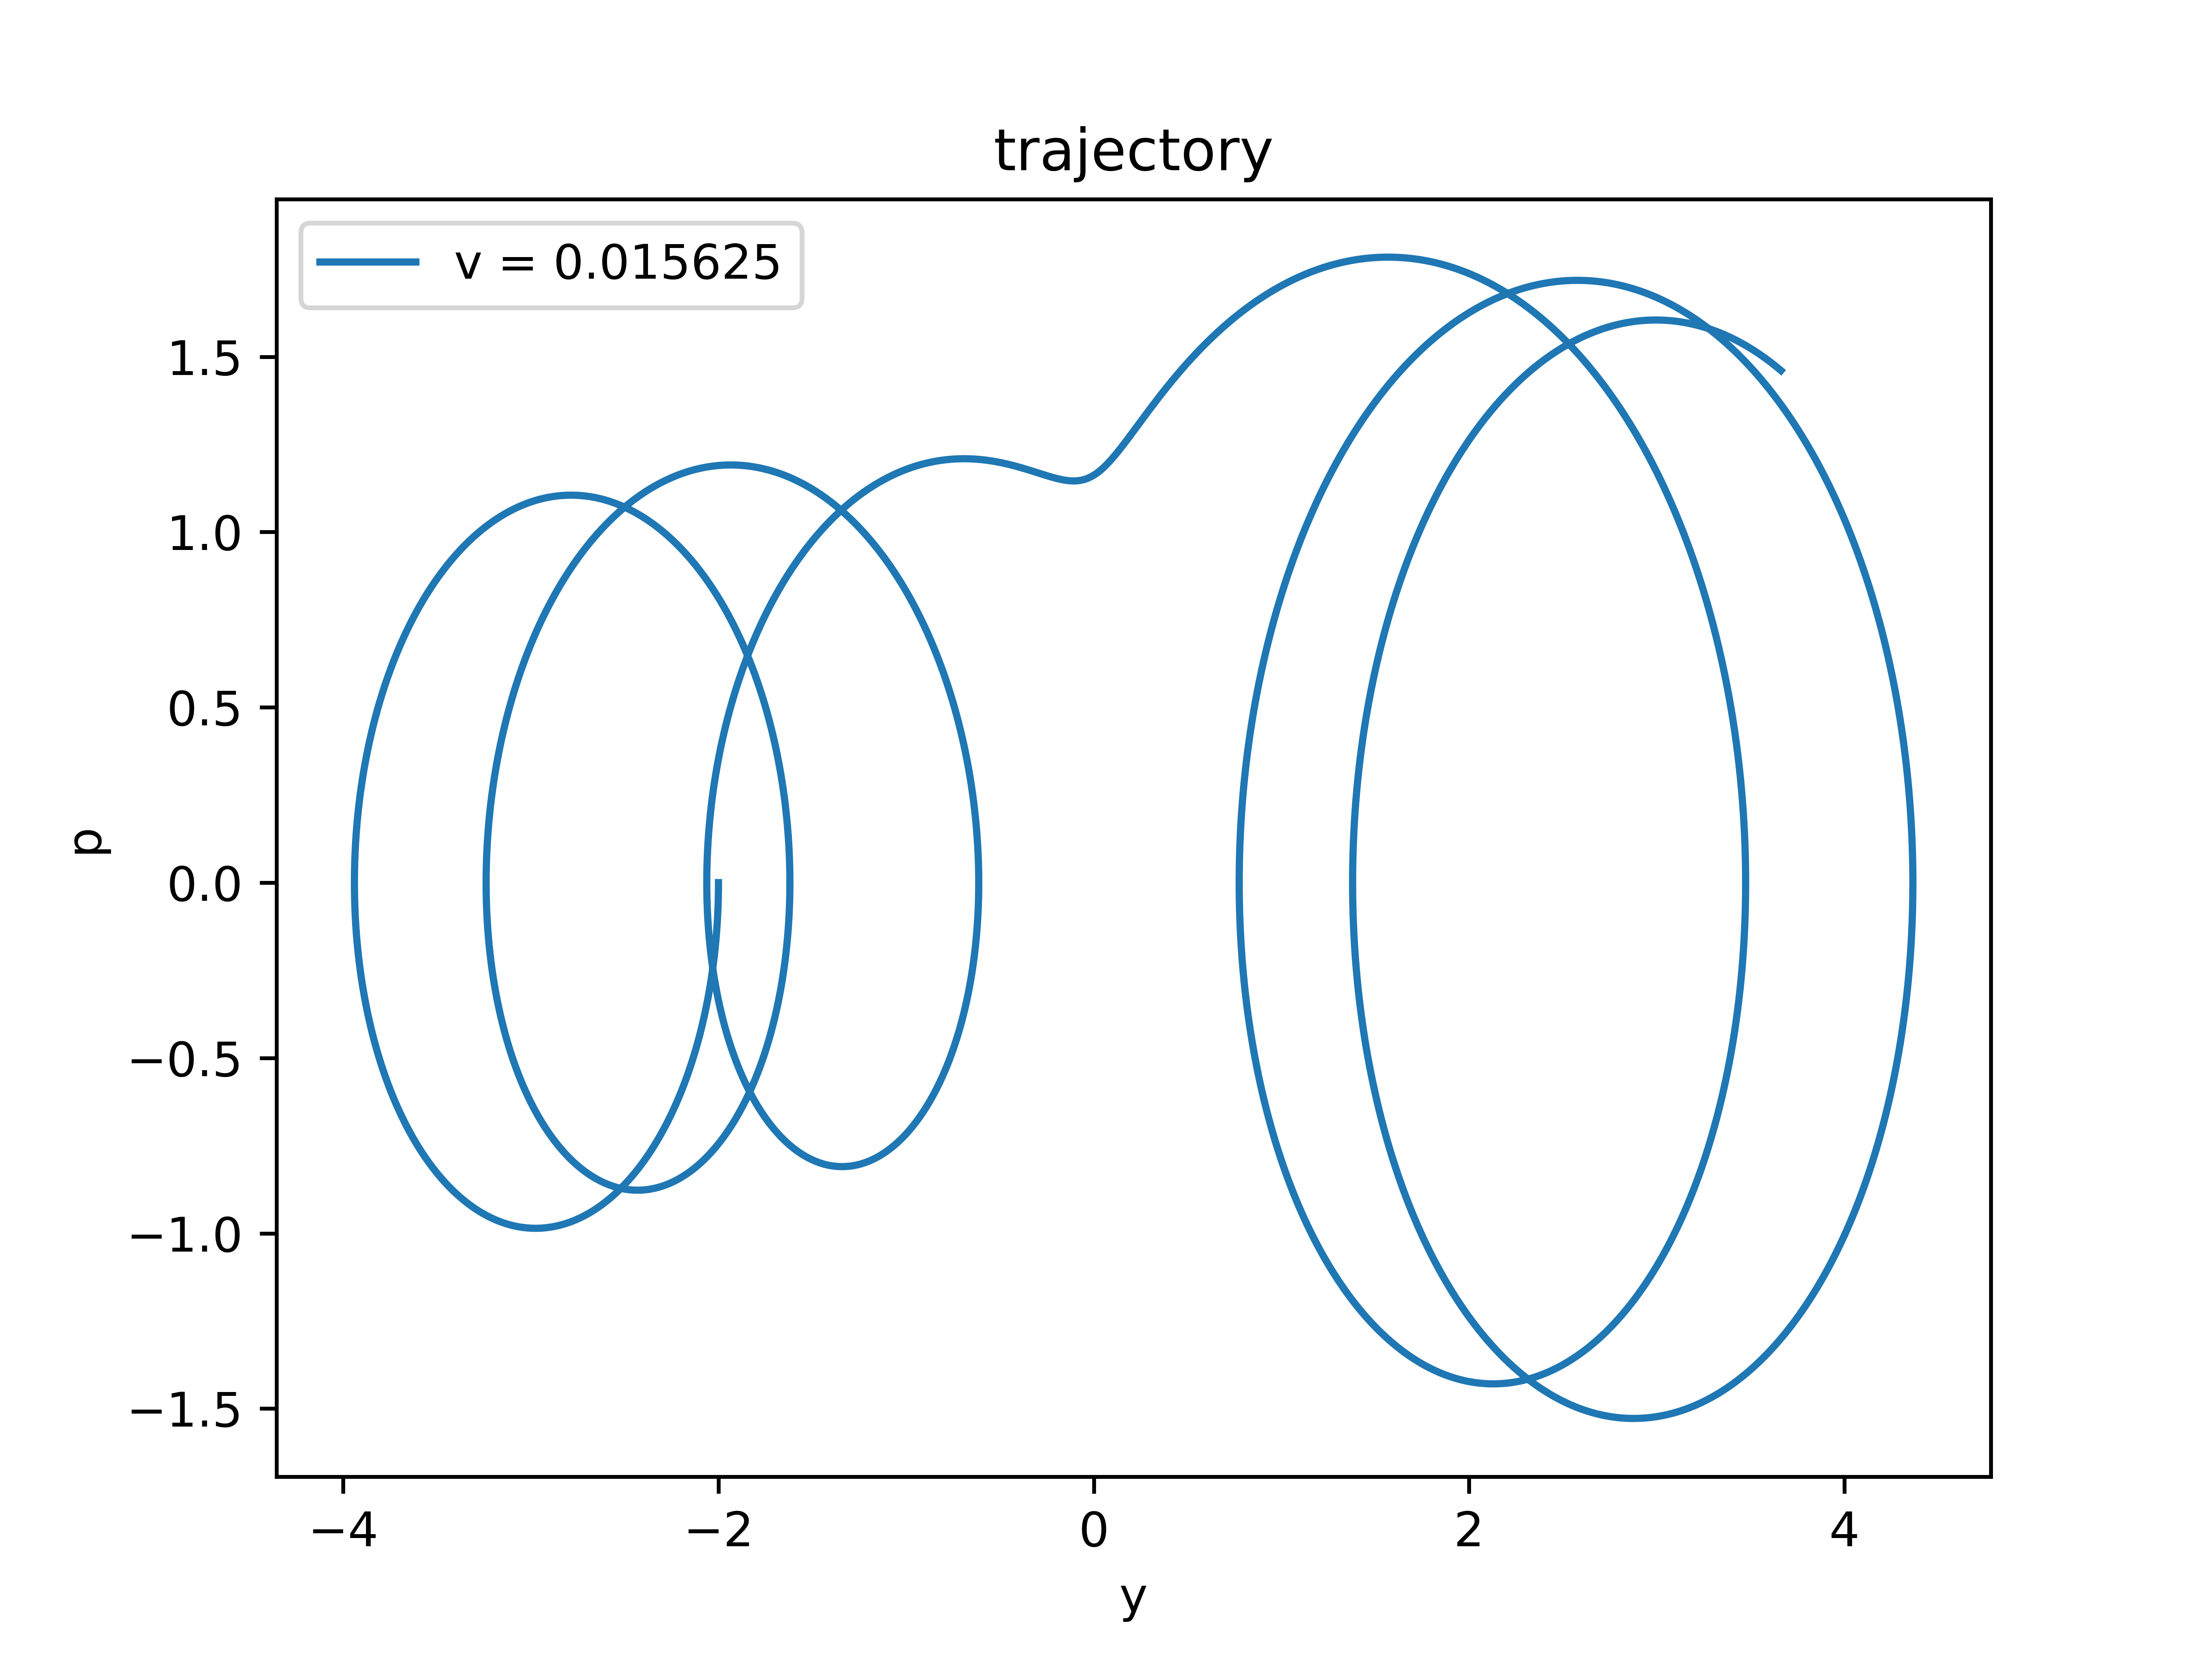
\includegraphics[scale=0.5]{3_traj_v=0_015625.png} & 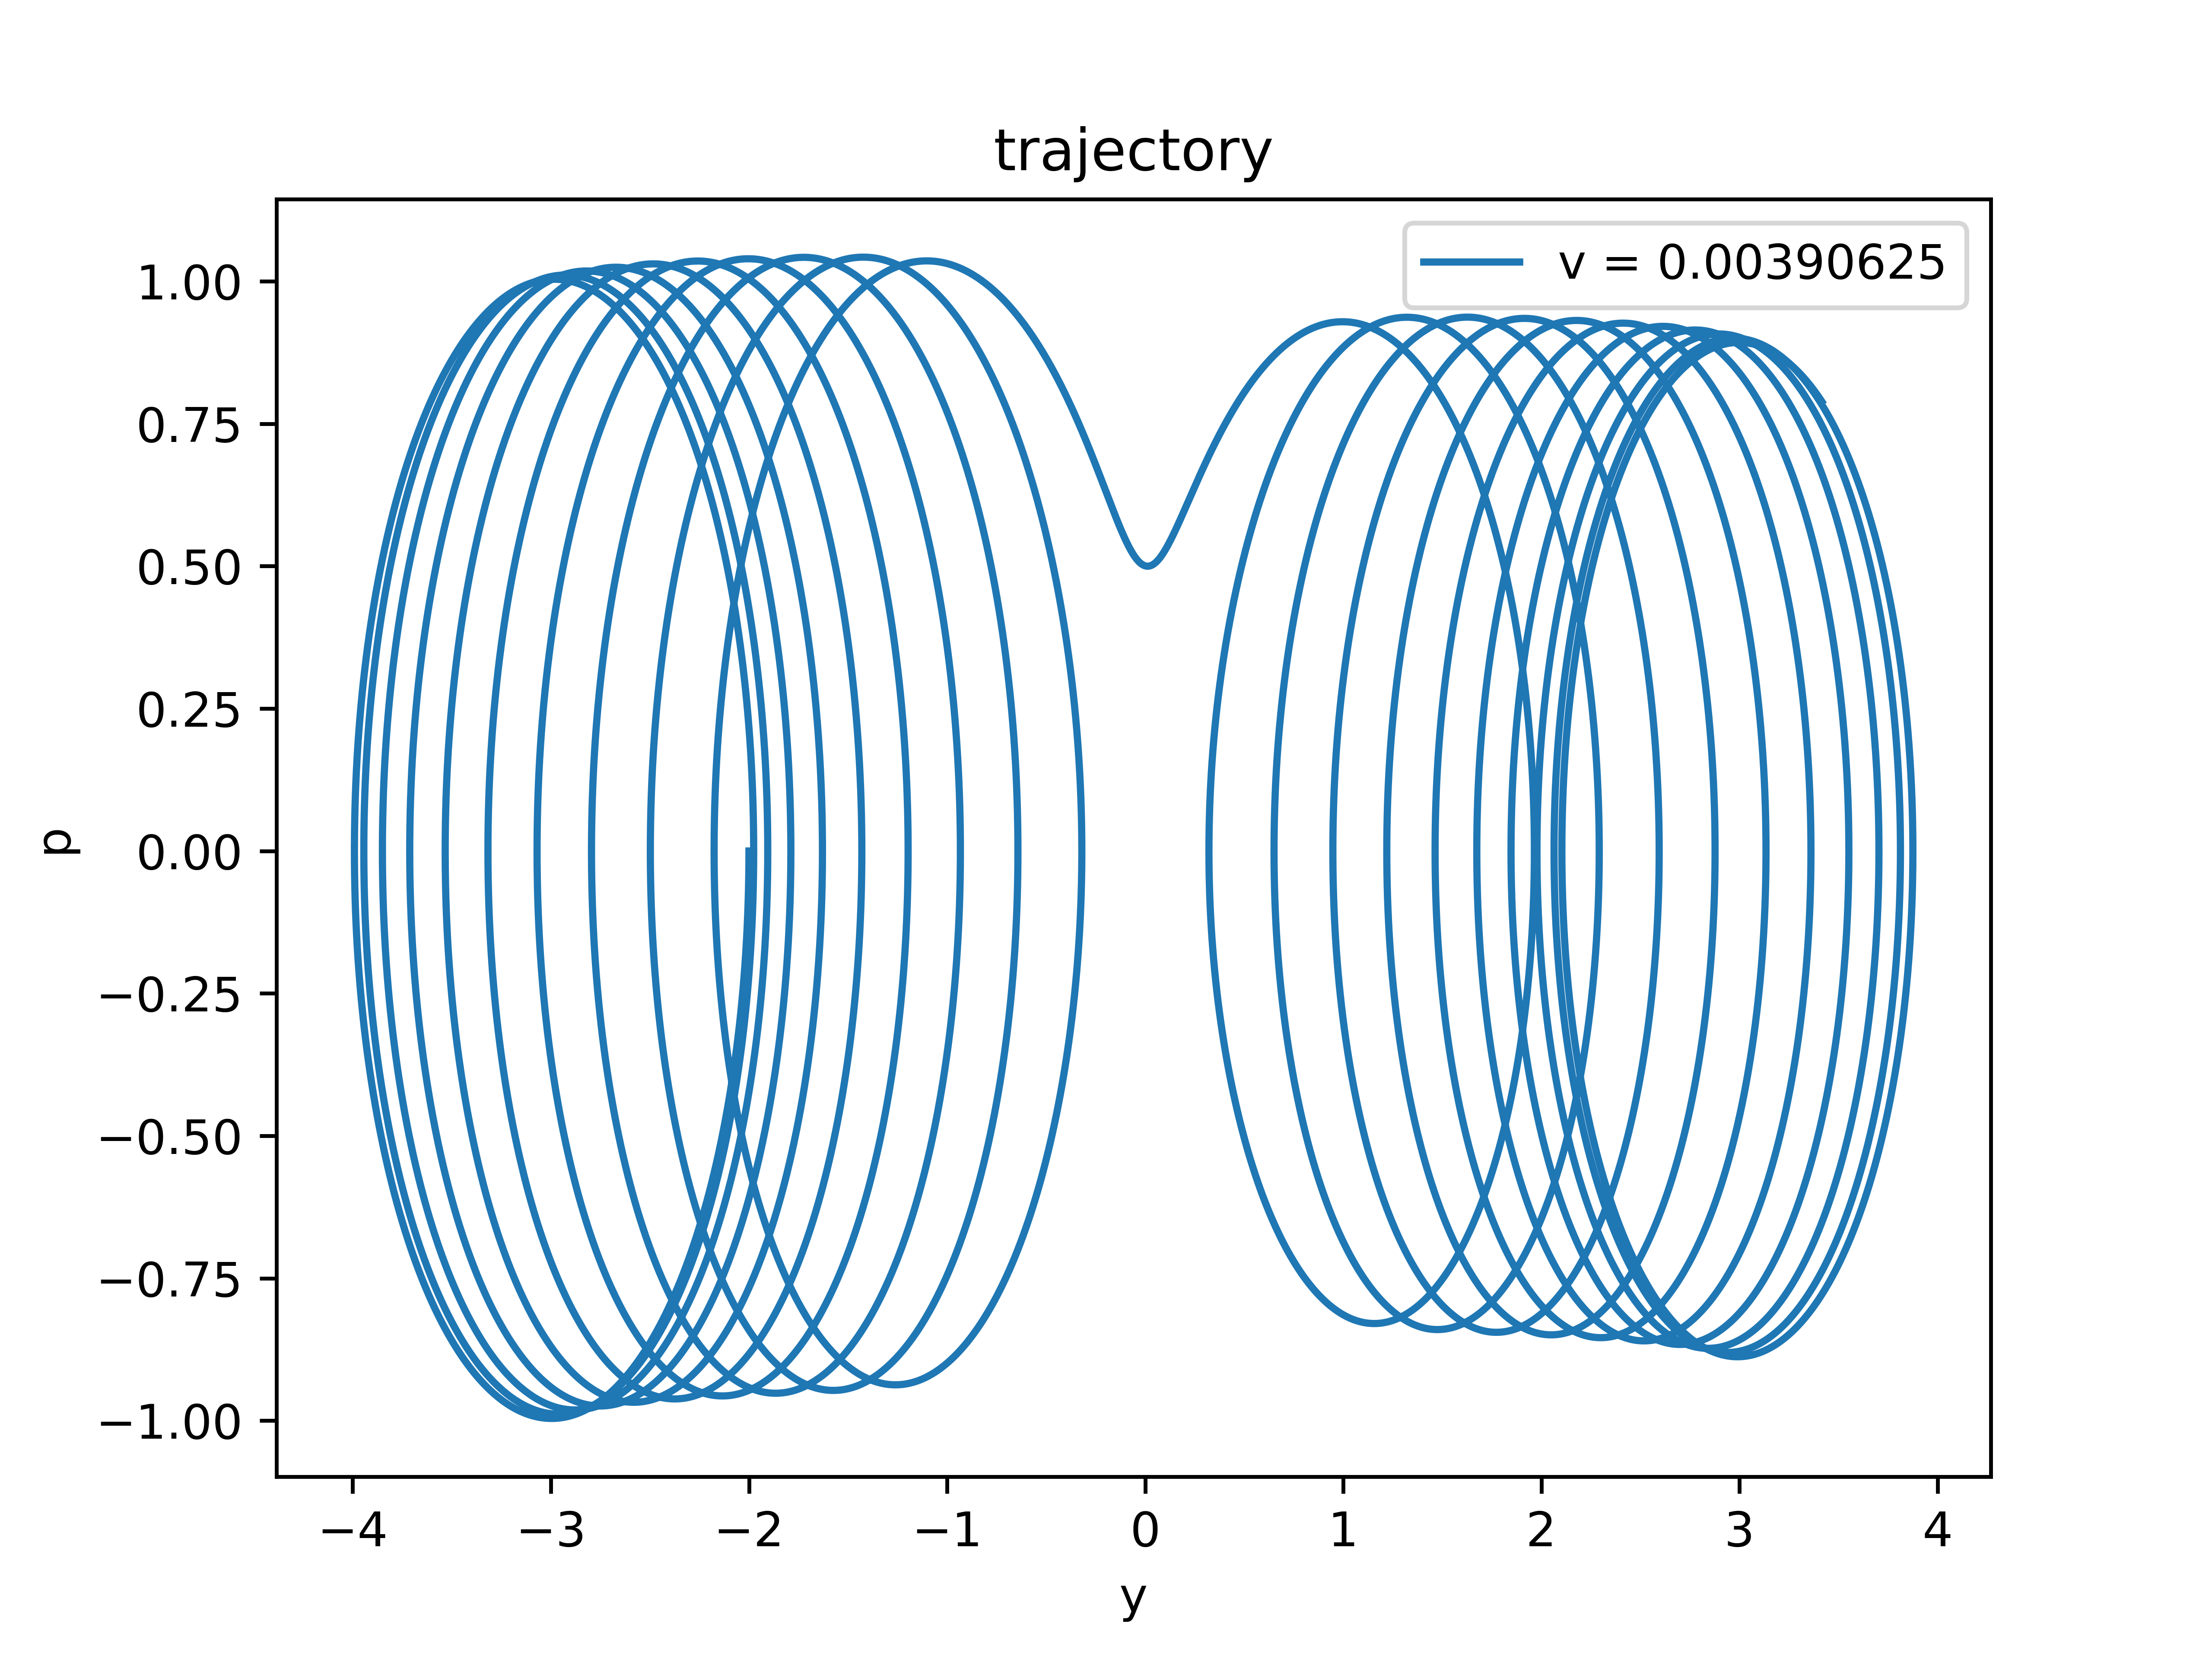
\includegraphics[scale=0.5]{3_traj_v=0_00390625.png}
        \end{tabular}
        \caption{$g$以不同速度变化时相轨线的变化}
        \label{g change}
    \end{table}
    \par 
    比较麻烦的是绝热不变量的计算, 需要准确计算对应的$y_\mr{min}, y_\mr{max}$. 考虑如下流程, 首先\textbf{判断}
    势能有几个稳定极值点, 若有一个: 找到能量极小值, 数值求出经典拐点, 使用Chebyshev积分计算绝热不变量; 若有两个, 
    计算两个拐点之间的局域极大值$E_M$, \textbf{判断}总能量$E$与$E_M$的大小关系, 若$E<E_M$进一步
    \textbf{判断}系统当前处于哪一个能量极小值区域, 找到对应区域后求出局域极小值, 再利用数值算法求出拐点,
    进而计算绝热不变量;
    若$E > E_M$那么在局域极大值两侧分别数值求根, 计算绝热不变量. 上述流程在代码3\_trajectory.cpp中实现了,
     主要逻辑可以参考:
     \begin{lstlisting}
        E = energy(y[0], p[0]);
        if (force(y_l, v, t) * force(y_r, v, t) > delta) {
          // only has one stable point
          double y_m = golden_section_opt(potential_inverse, -10.0, 10.0, 1e-4);
          y_min = dekker_root(tunnel_points, -10.0, y_m, 1e-6);
          y_max = dekker_root(tunnel_points, y_m, +10.0, 1e-6);
          J = chebyshev_second_integral(J_func, y_min, y_max, 1e3);
        } else if (force(y_l, v, t) * force(y_r, v, t) < -delta) {
          // has two stable points
          double y_M = golden_section_opt(potential, y_l[0], y_r[0], 1e-4);
          double E_M = potential(y_M);
          if (E_M - E > delta) {
            // can not cross the barrier
            if (y[0] < y_M) {
              double y_m = golden_section_opt(potential_inverse, -10, y_M, 1e-4);
              y_min = dekker_root(tunnel_points, -10, y_m, 1e-6);
              y_max = dekker_root(tunnel_points, y_m, y_M, 1e-6);
              J = chebyshev_second_integral(J_func, y_min, y_max, 1e3);
            } else if (y[0] > y_M) {
              double y_m = golden_section_opt(potential_inverse, y_M, 10, 1e-4);
              y_min = dekker_root(tunnel_points, y_M, y_m, 1e-6);
              y_max = dekker_root(tunnel_points, y_m, 10, 1e-6);
              J = chebyshev_second_integral(J_func, y_min, y_max, 1e3);
            }
          } else if (E - E_M > delta) {
            y_min = dekker_root(tunnel_points, -10, y_M, 1e-6);
            y_max = dekker_root(tunnel_points, y_M, 10, 1e-6);
            J = chebyshev_second_integral(J_func, y_min, y_max, 1e3);
          }
        }
     \end{lstlisting}
     \par 
     绝热不变量随$g$的变化展示在表 中:
     \begin{table}[htbp]
        \centering
        \begin{tabular}[htbp]{cc}
            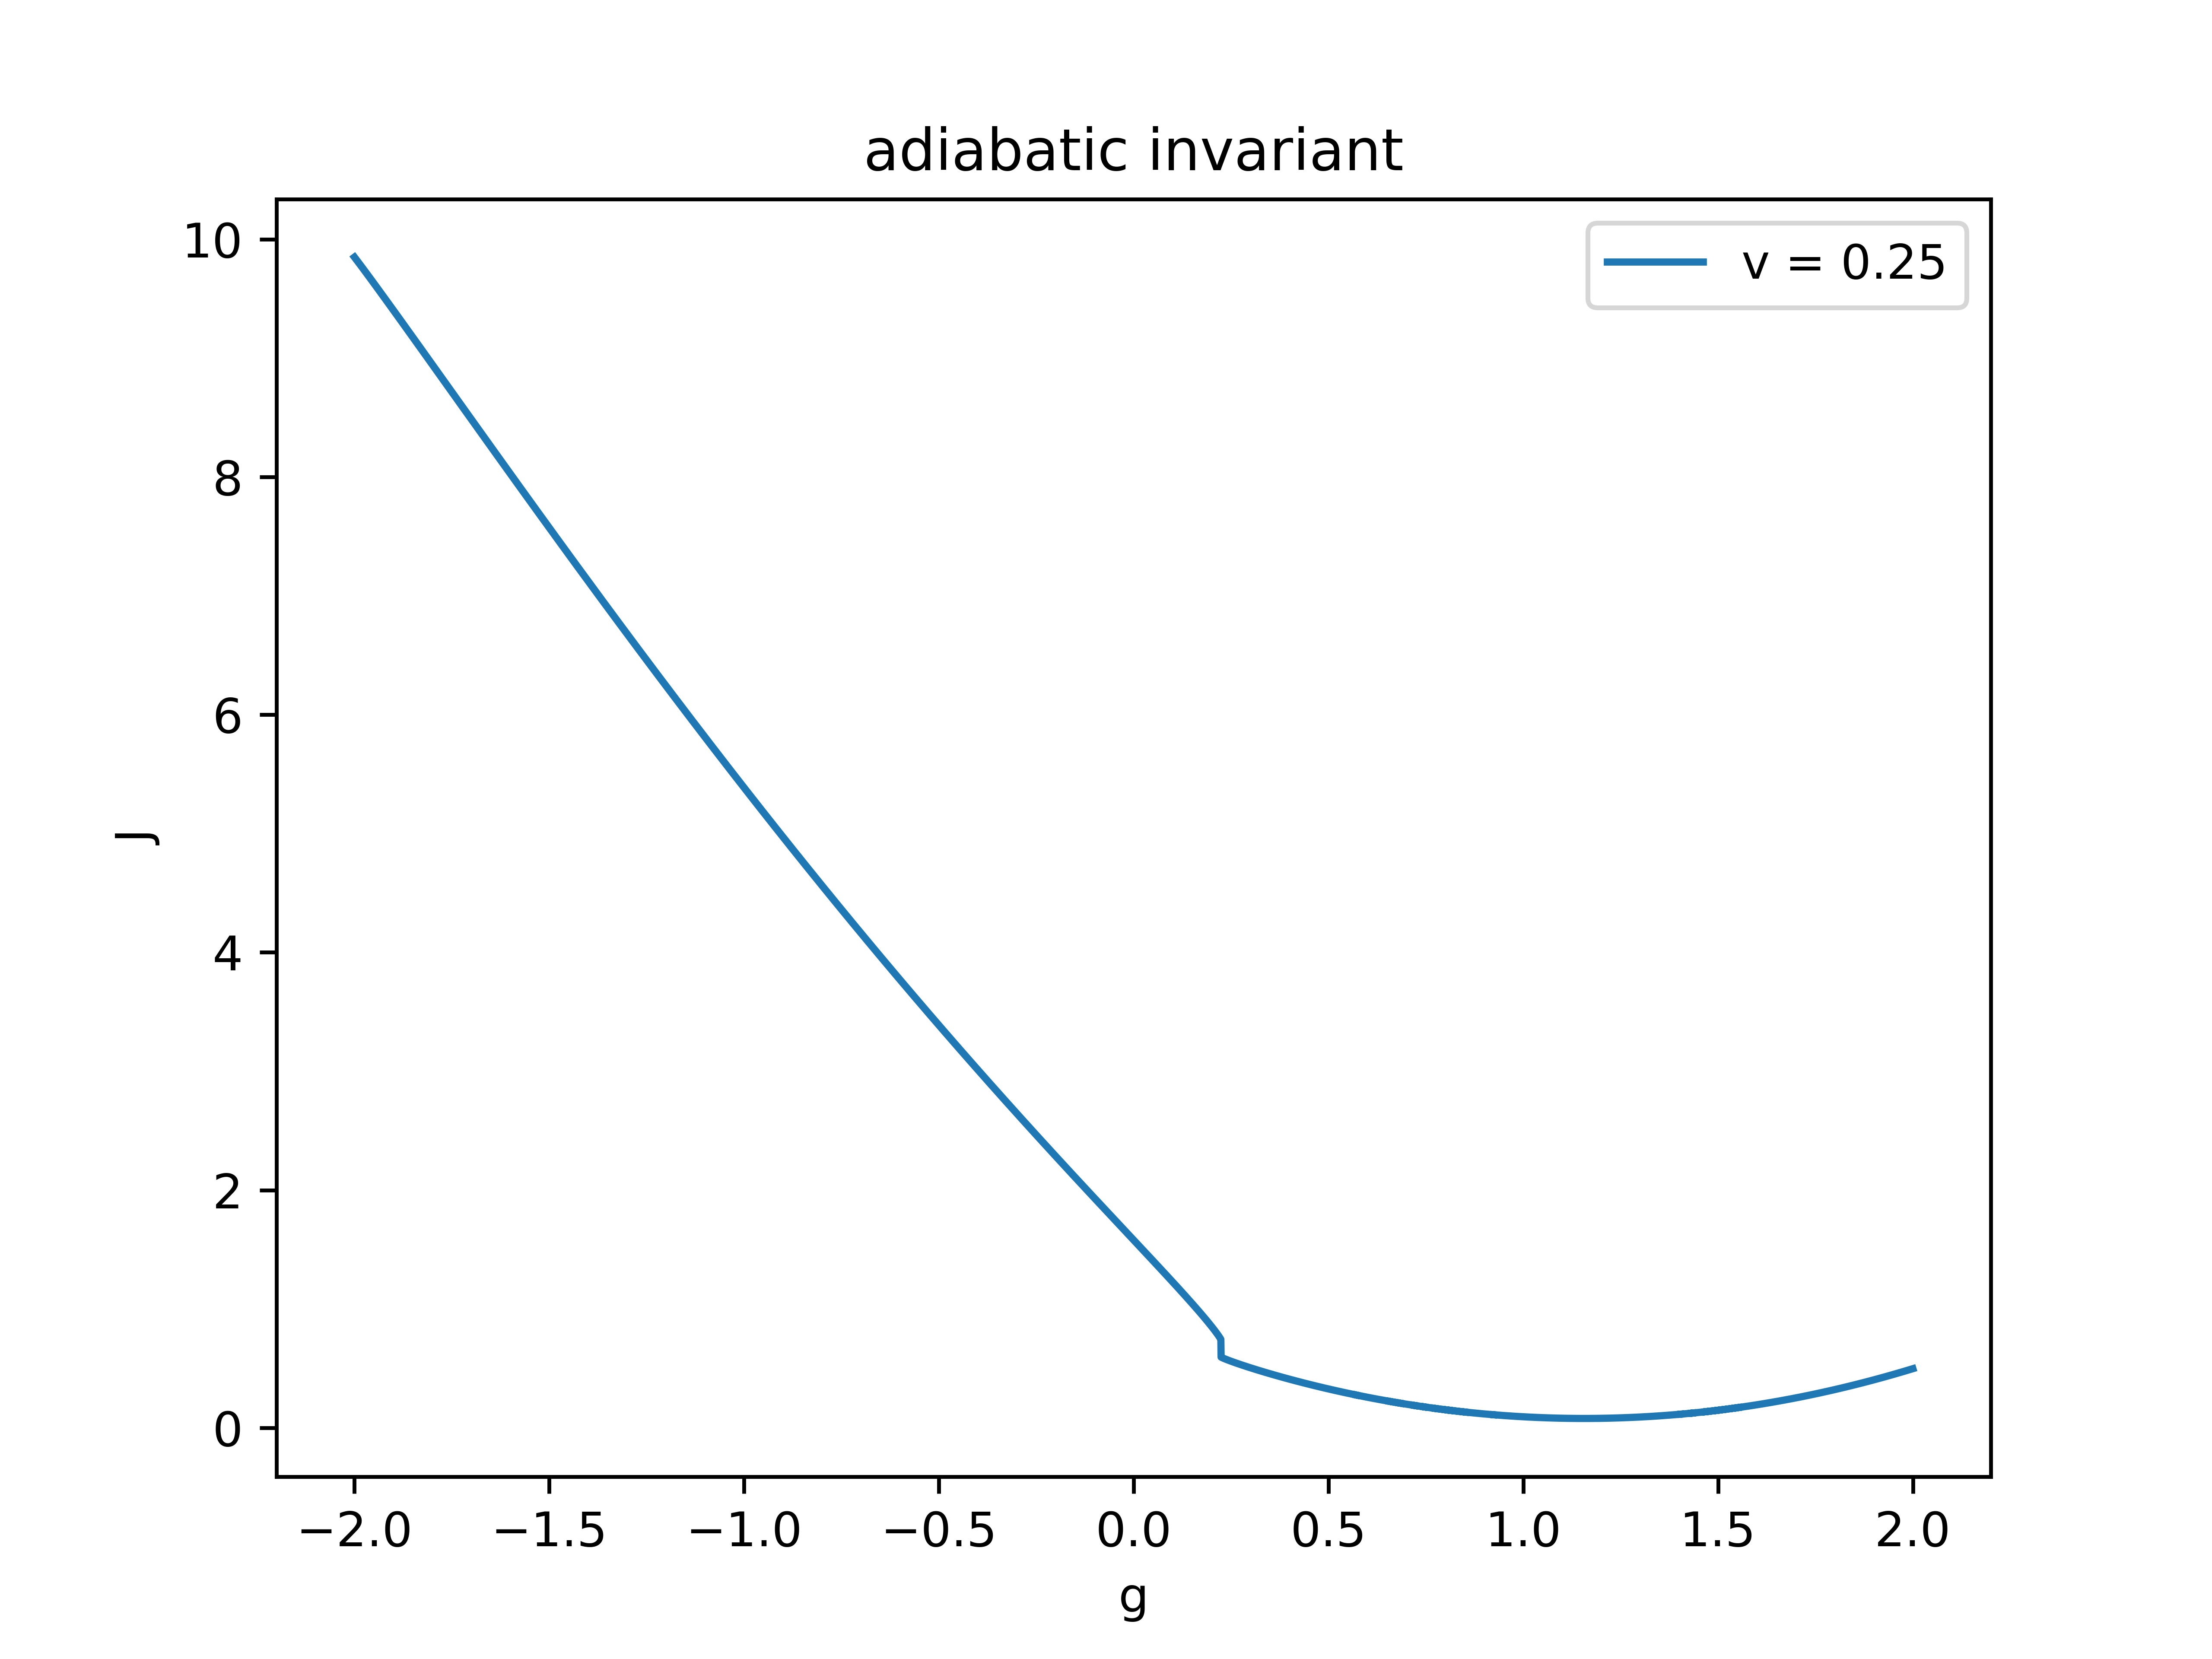
\includegraphics[scale=0.5]{3_ad_invr_v=0_25.png} & 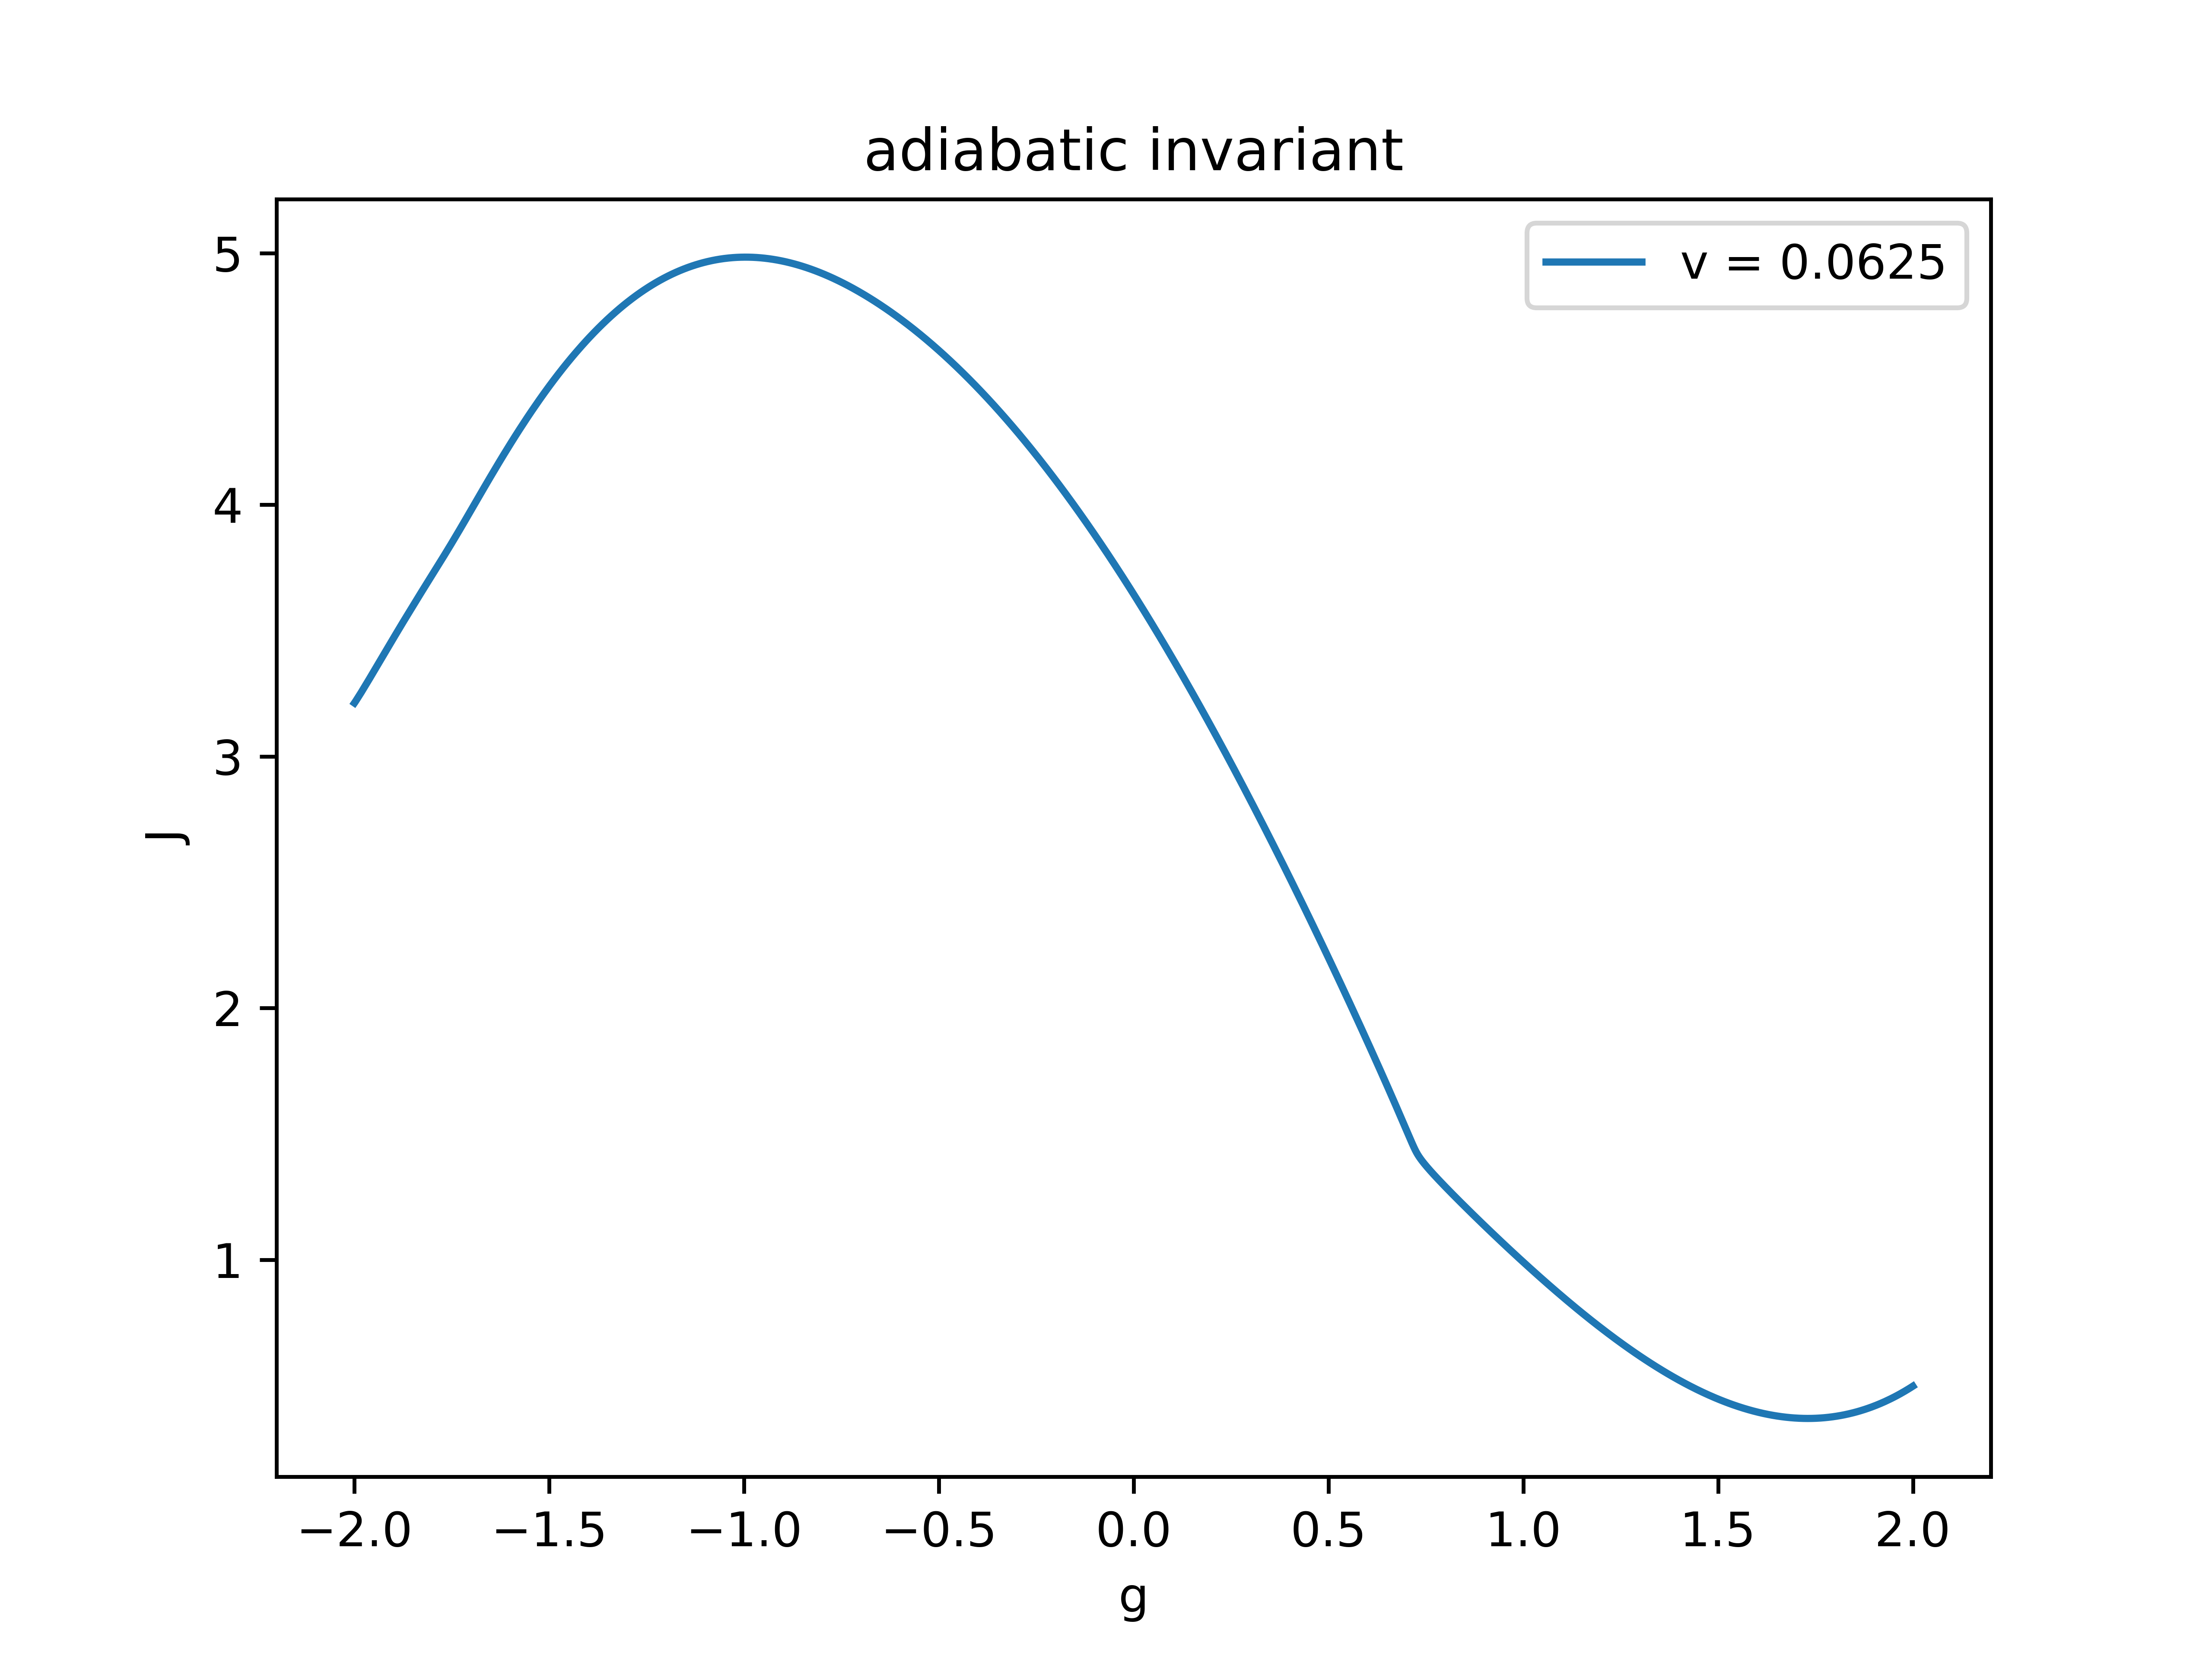
\includegraphics[scale=0.5]{3_ad_invr_v=0_0625.png} \\
            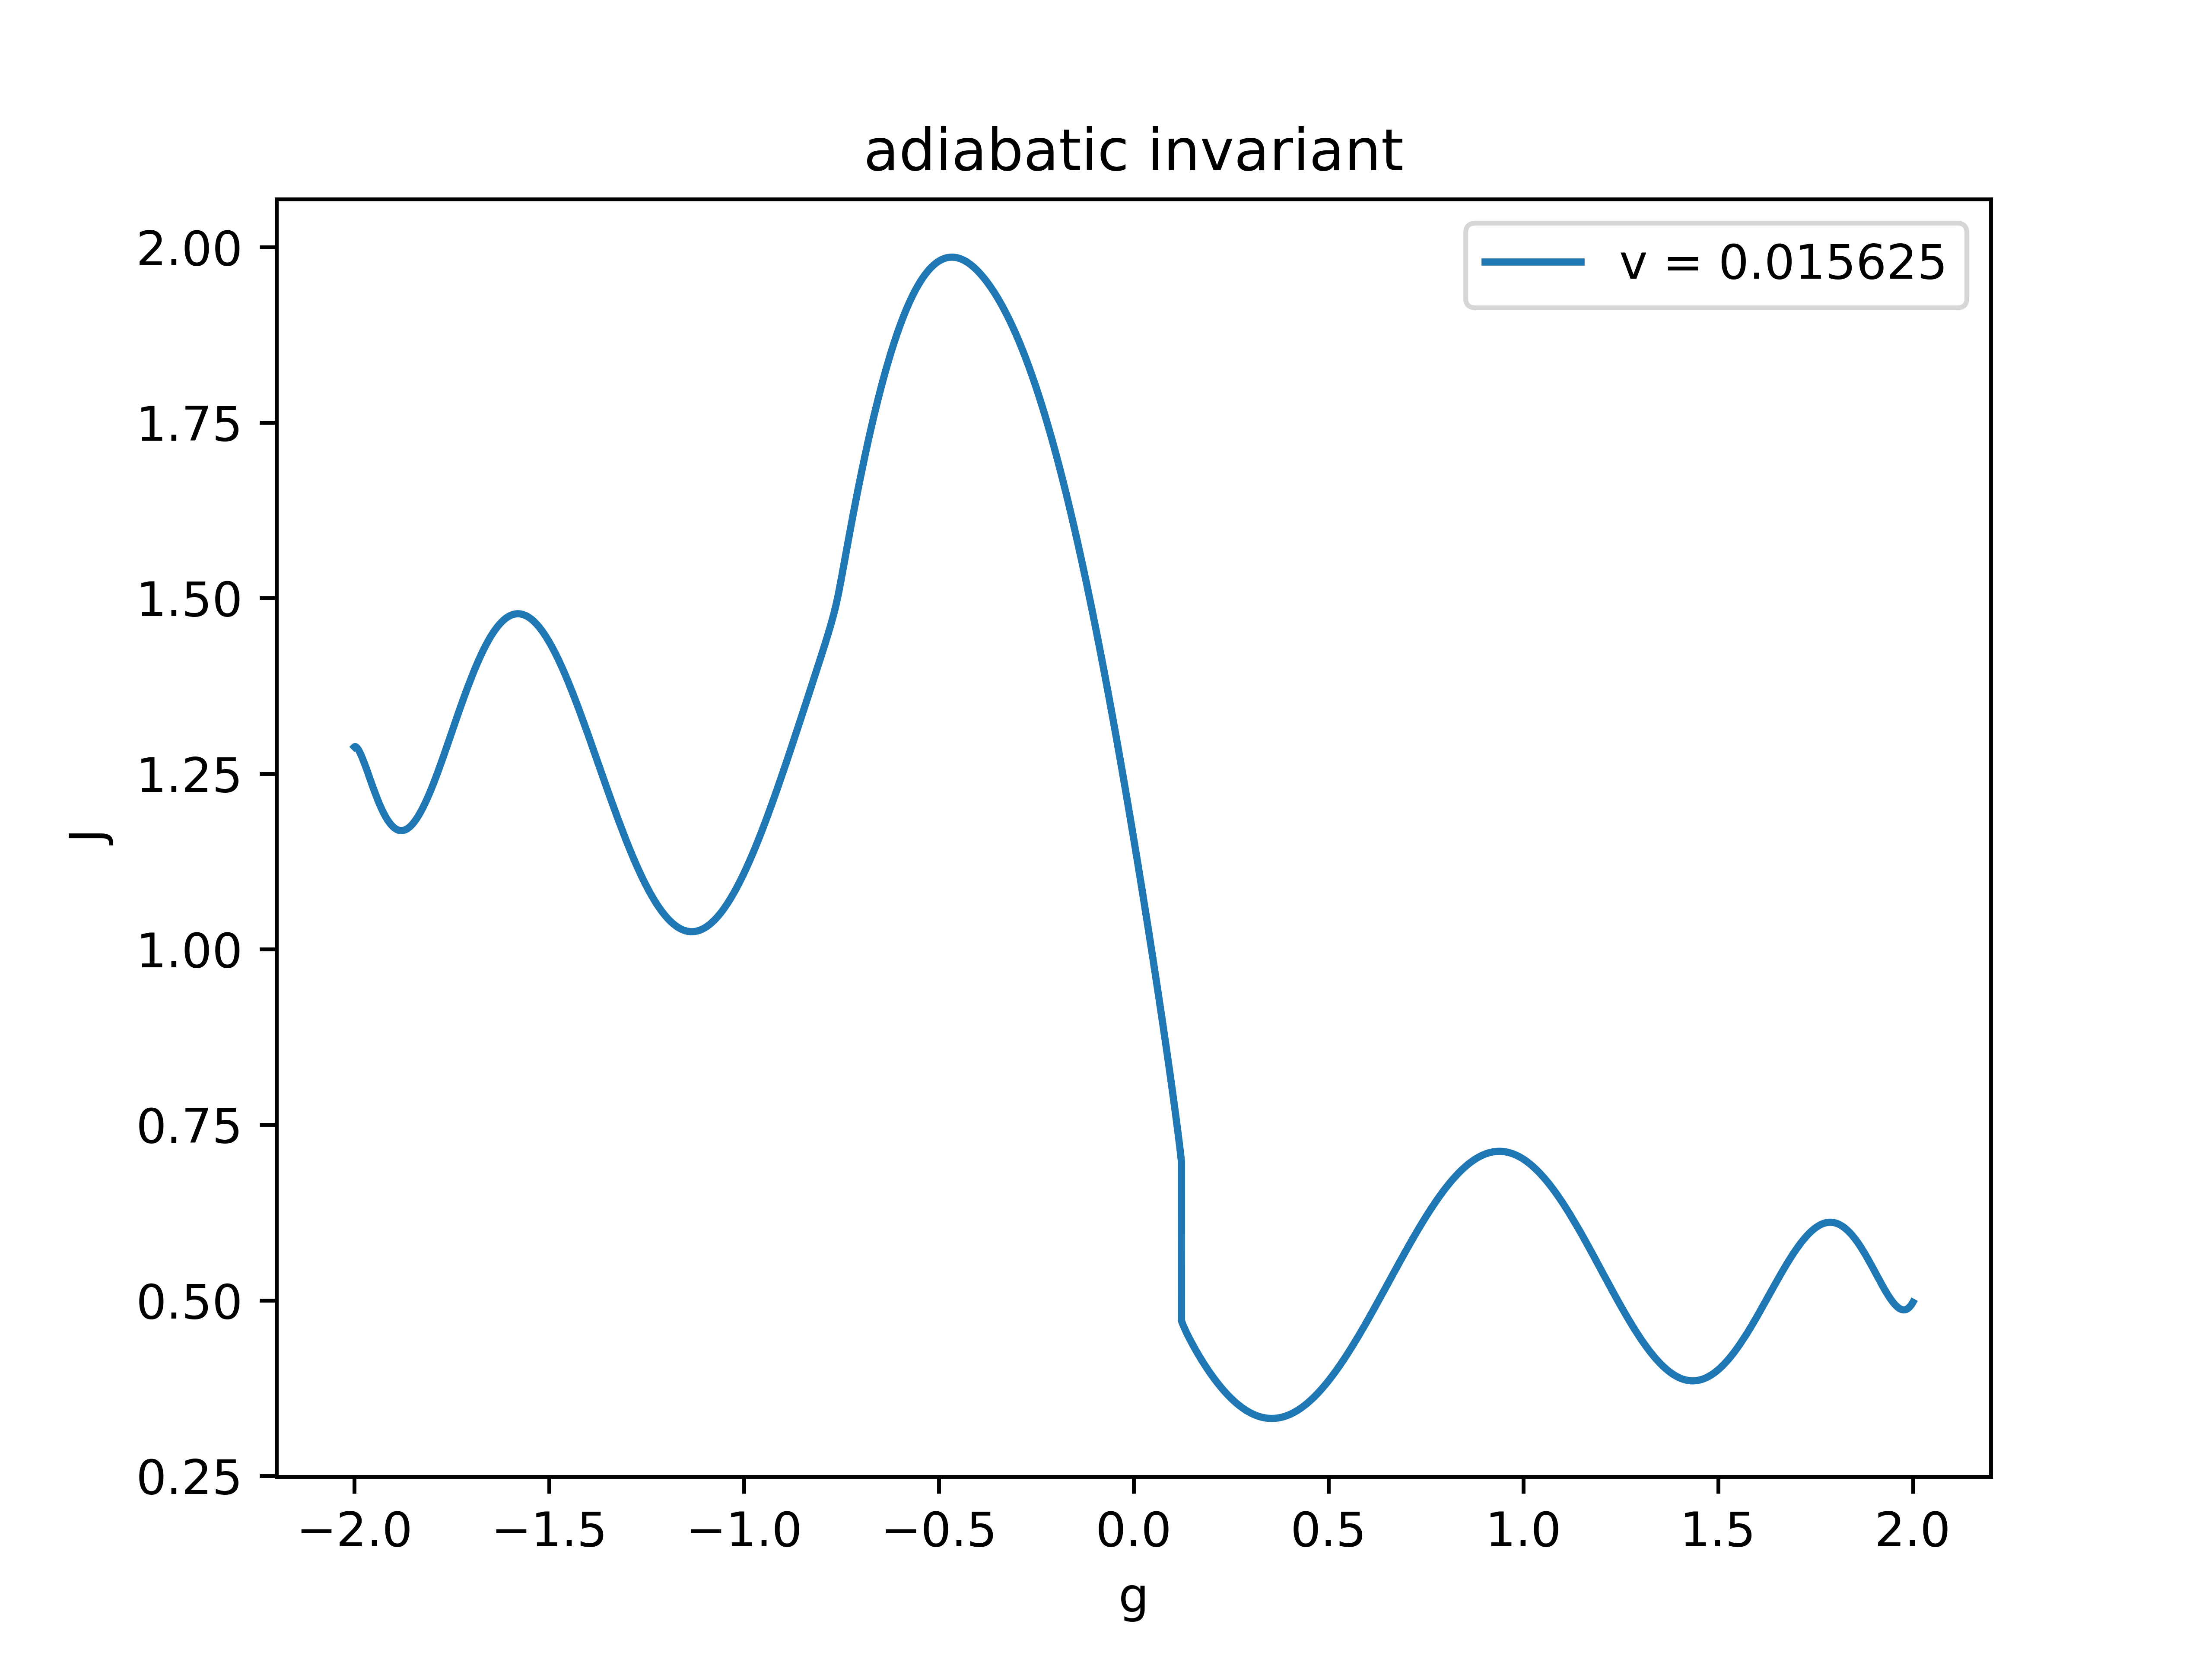
\includegraphics[scale=0.5]{3_ad_invr_v=0_015625.png} & 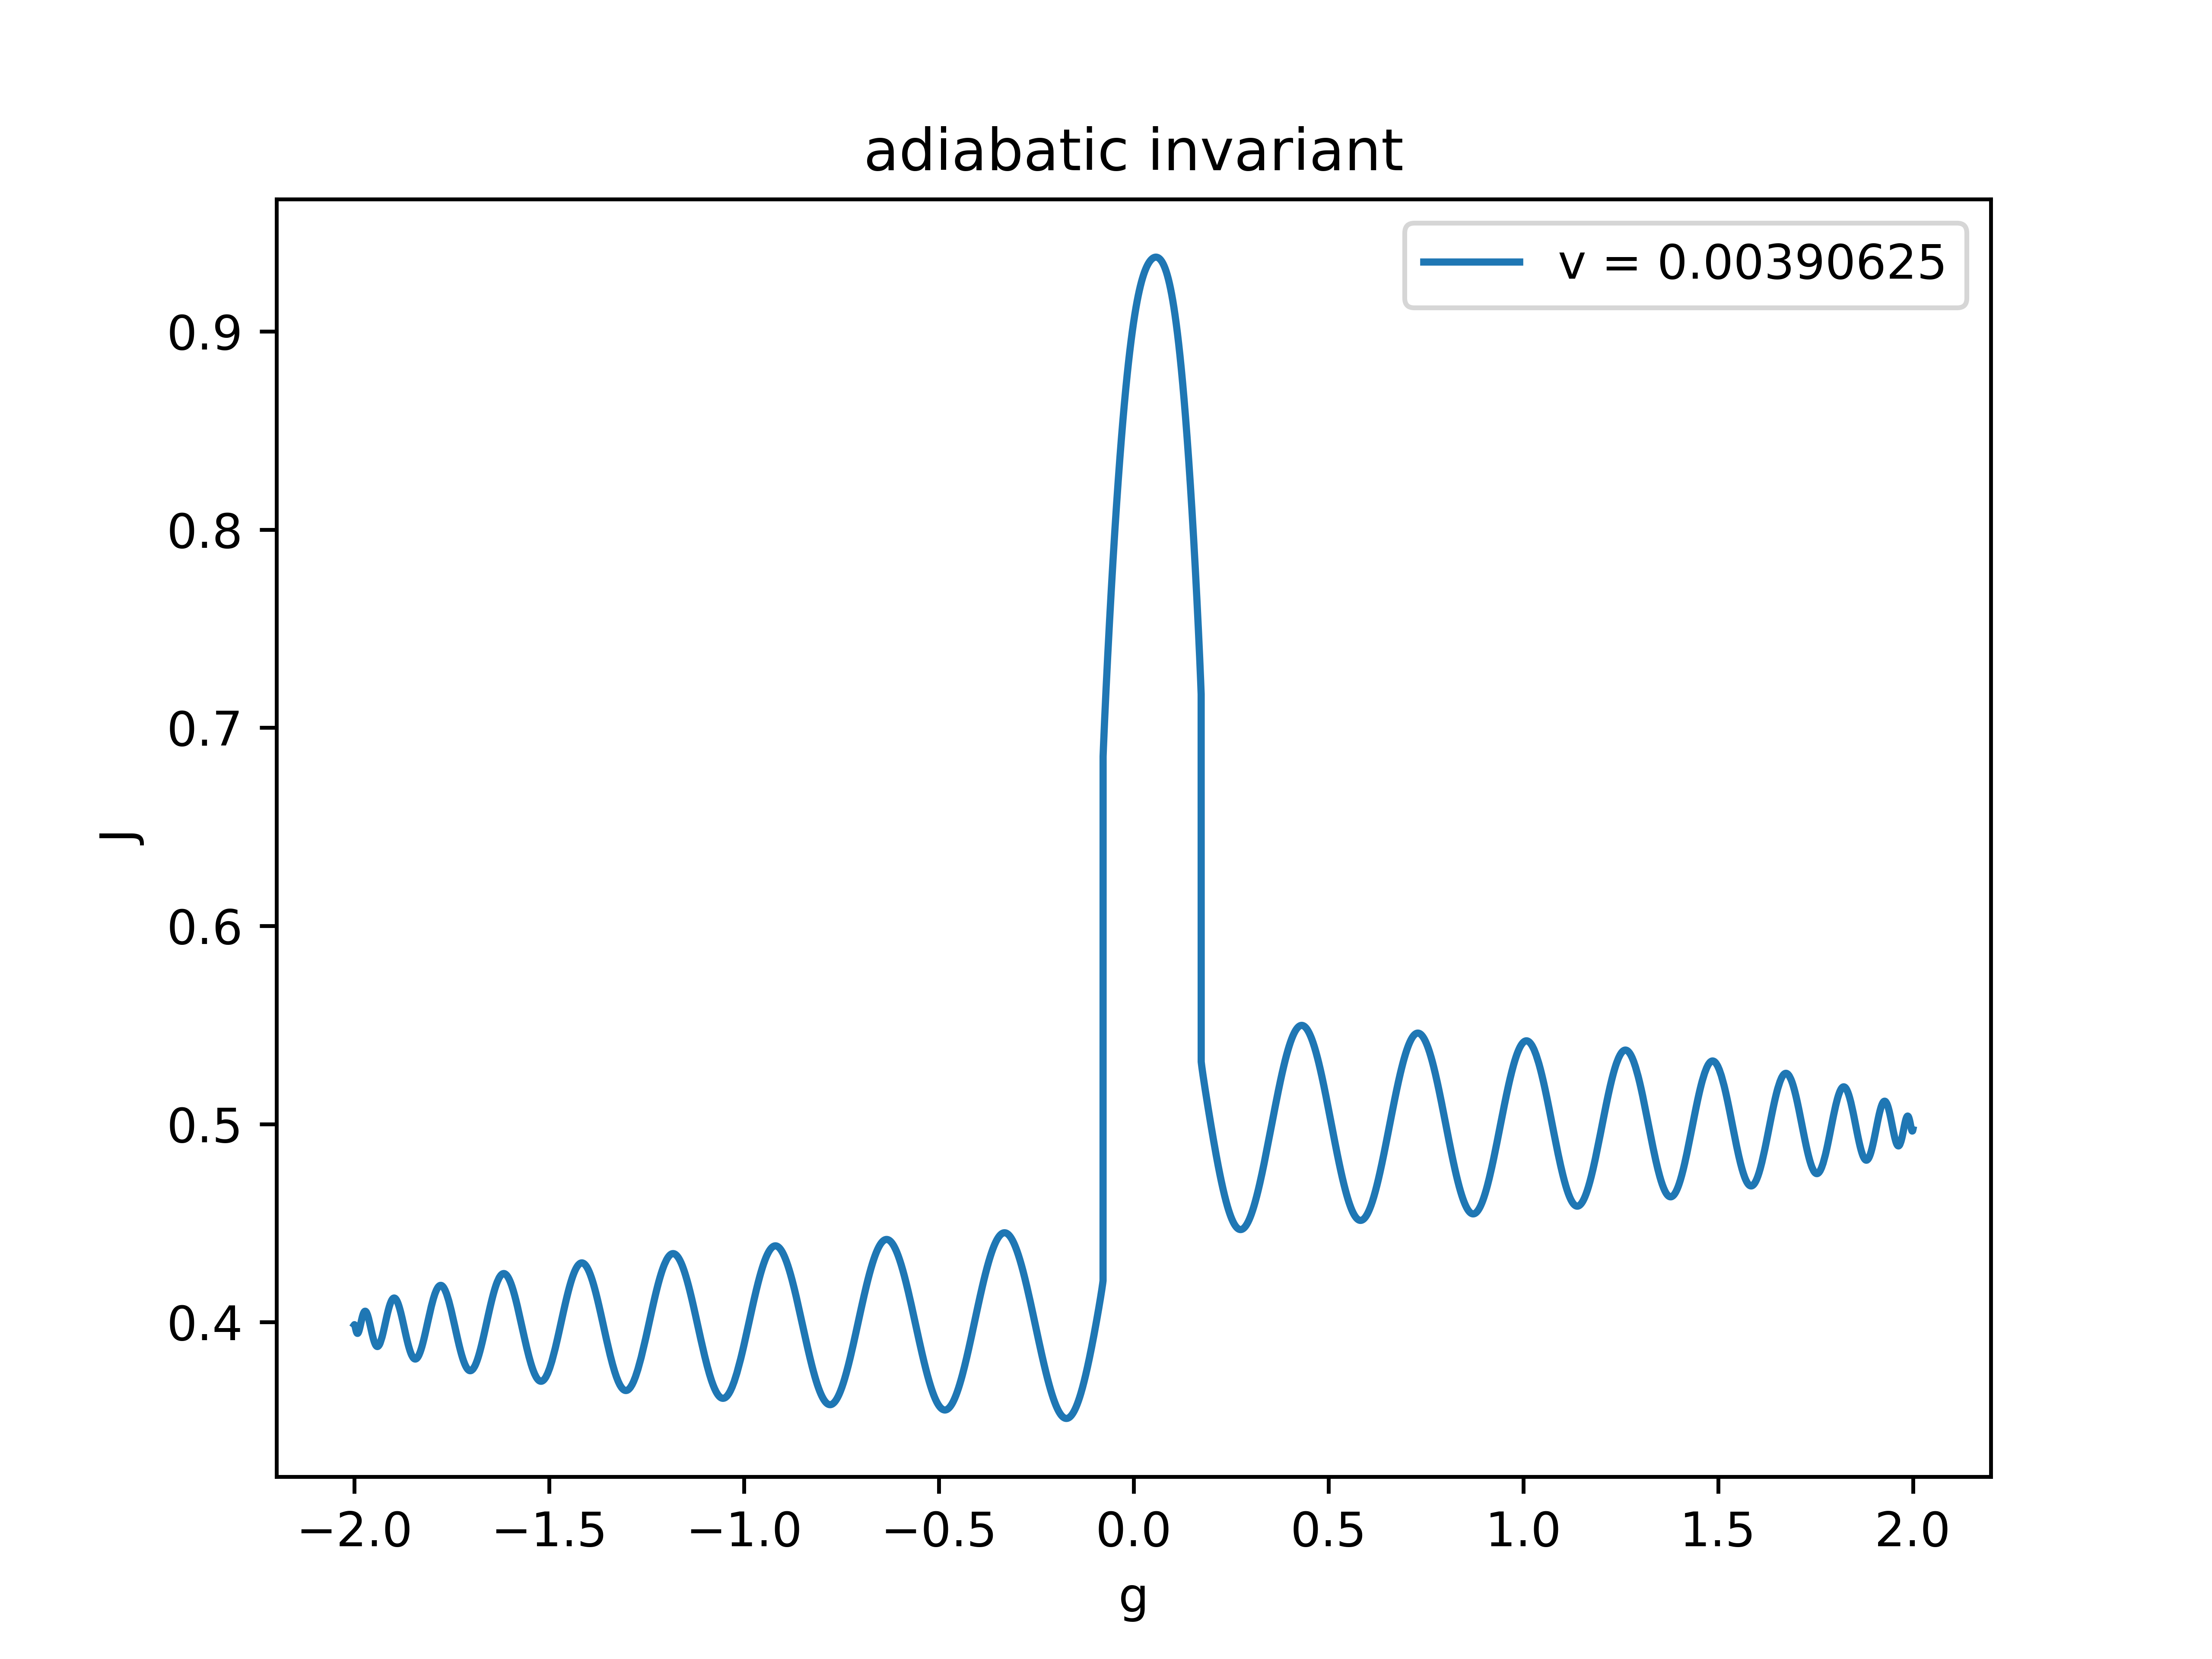
\includegraphics[scale=0.5]{3_ad_invr_v=0_00390625.png}
        \end{tabular}
        \caption{$g$以不同速度变化时绝热不变量$J$的变化}
        \label{g change J}
    \end{table}
    \par 
    当$g$这个参数改变时, 系统会从一个单侧的不对称势阱变成不对称双势阱, 再变成另一侧的不对称单势阱. 
    可以看到系统的绝热不变量在外参数变化足够缓慢时总是局部地稳定, 只有在系统跨越势垒前往新的平衡位置的时候才会剧烈变化.
    \subsection{Berry相位}
    对于参数随时间的周期变化, 可以定义周期内的Berry相位, 将整个演化过程的初态和末态分别定义为$(p_i, q_i),\,(p_f,q_f)$,
    Berry相位记为:
    \begin{equation}
        \phi_B = \left[\omega(t_i)\int_{(p_i, q_i)}^{(p_f,q_f)}\d t - \int_{t_i}^{t_f}\omega(t)\d t\right] \text{mod}2\pi
    \end{equation}
    对上面的定义式进行简单的分析, $\omega(t_i)$代表了初始时刻的系统的运动角频率, $(p_i, q_i)\to(p_f, q_f)$对
    时间的积分表示固定系统含时参数为初态的参数, 在能量守恒的情况下演化到末态所需要的时间. 
    这看起来好像不太可能, 当参数随时间变化时, 轨线可能会偏离初始位置很远, 甚至到达新的平衡点附近运动,
    如果参数变化地足够缓慢, 相轨迹可能充满相空间的某个区域, 怎么保证在外参数变化一个周期后, 
    轨线回到初始位置“附近”并落在初态参数对应的轨线上? 事实上对于一维系统(或许可以推广到完全可积系统?), 
    系统的能量和绝热不变量一一对应(这当然是含时参数固定不变的情况下), 由绝热定理知当参数缓慢变化时绝热不变量不变, 
    那么当参数演化一个周期回到初态后, 系统的末态能量和初态一致, 这样就保证了初态和末态系统在同一个轨线上.
    \par
    而对$\omega$的积分表示了对相空间一条给定轨迹上的积分. 数值实验时考虑按照题目给定的初始条件演化一条相空间中的轨迹, 
    然后选取轨线上的点计算对应位置的频率, 这其中涉及到了经典拐点的求解, 使用的方法应该与之前类似. 但是也有很多细节上的
    问题, 比如要特别注意$x=0$时势能函数会出现不可导的点, 那么需要对力函数进行修改, 在$\frac{0}{0}$的分数分子分母上
    加上一个小量(要远小于程序中使用的数值积分、求根、求极值算法的误差), 同时保证趋于零的极限值正确:
    \begin{lstlisting}
        double force(double *y) {
            double dist = 0;
            dist = sqrt(x * x + y[0] * y[0]);
            // to aviod divided by  zero
            if (y[0] > 0) {
                return -k * (dist - l) * (y[0] + delta) / (dist + delta) - m * g;
            } else {
             return -k * (dist - l) * (y[0] - delta) / (dist - delta) - m * g;
            }
        }
    \end{lstlisting}
    此外还在其他地方使用类似的方法处理了数值误差可能带来的影响. 
    \par 
    事实上在求解这一问的时候遇到了相当的困难, Berry相位无论怎么计算都不趋于0. 仔细分析了一下问题可能出现的原因, 
    最后发现计算周期的Chebyshev积分在初始时刻不能给出准确值, 大约有千分之一的误差, 这是计算Berry相位无法接受的, 
    仔细检查后得出结论, 是因为数值求根的精度没有设置合适导致积分限有很小的误差, 在Chebyshev积分时每一个节点
    的选取都会产生误差, 这些误差加和造成了明显的误差, 将数值求根的精度提高之后明显改善了这一现象. 
    \par
    这两问的程序参见4\_berry\_phase.cpp, 其中的初始值和相关参数在计算(4)(5)时需要改动, 编译使用compile4.bat与
    compile5.bat, 运行对应的可执行文件产对应的文本文件, 其中存储了时间、参数、位置和动量、绝热不变量和周期.
    计算从初态演化到末态时间的程序为4\_cal\_time.cpp, 需要手动输入文本文件的初末态位置和动量.
    计算Berry相位的程序为4\_plot.py, 会生成相应的图片和print Berry相位.
    \subsubsection{问题(4)}
    为了选择合适的参数$\nu$使得绝热不变量近似不变, 测试了不同的参数后觉得$\nu=0.0005$是一个不错的参数, 如果更小会使得
    程序运行时间略长(尽管会带来更好的绝热不变量的表现), 太大的话没法满足绝热不变量近似不变的要求.
    演化过程中的轨线、绝热不变量随参数的变化可以参见图\ref{4 traj}, \ref{4 g ad}, \ref{4 x ad}
    (说明一下为啥图片格式不统一, 有的图保存成png太大了就保存pdf了)
    \begin{figure}[htbp]
        \centering
        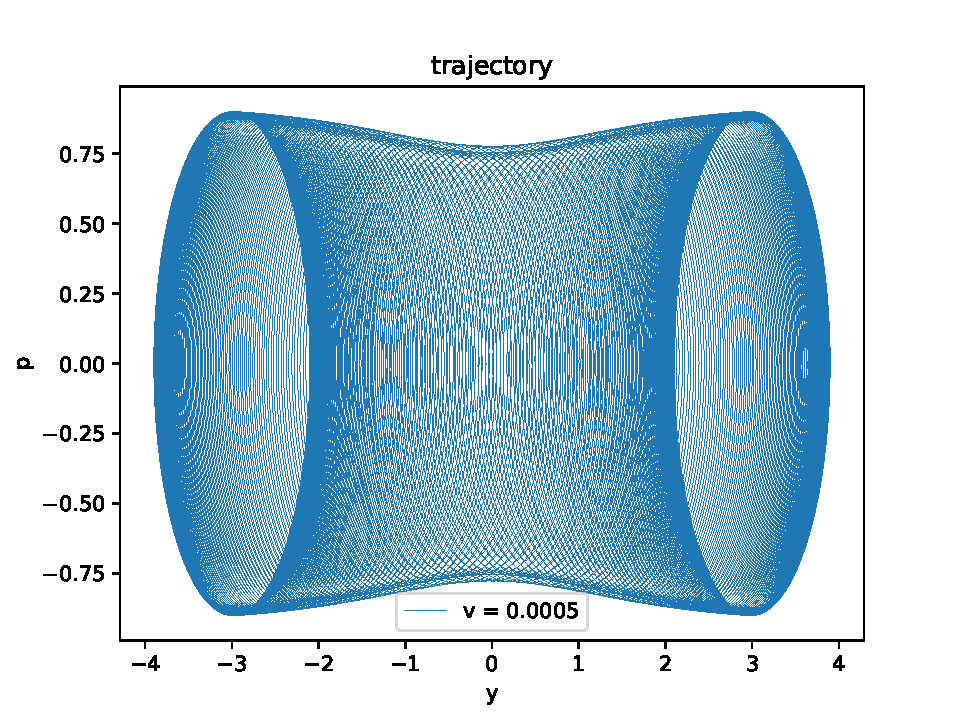
\includegraphics[scale=0.6]{4_traj_v=0_0005.pdf}
        \caption{参数变化一个周期时相空间轨线}
        \label{4 traj}
    \end{figure}
    \begin{figure}[htbp]
        \centering
        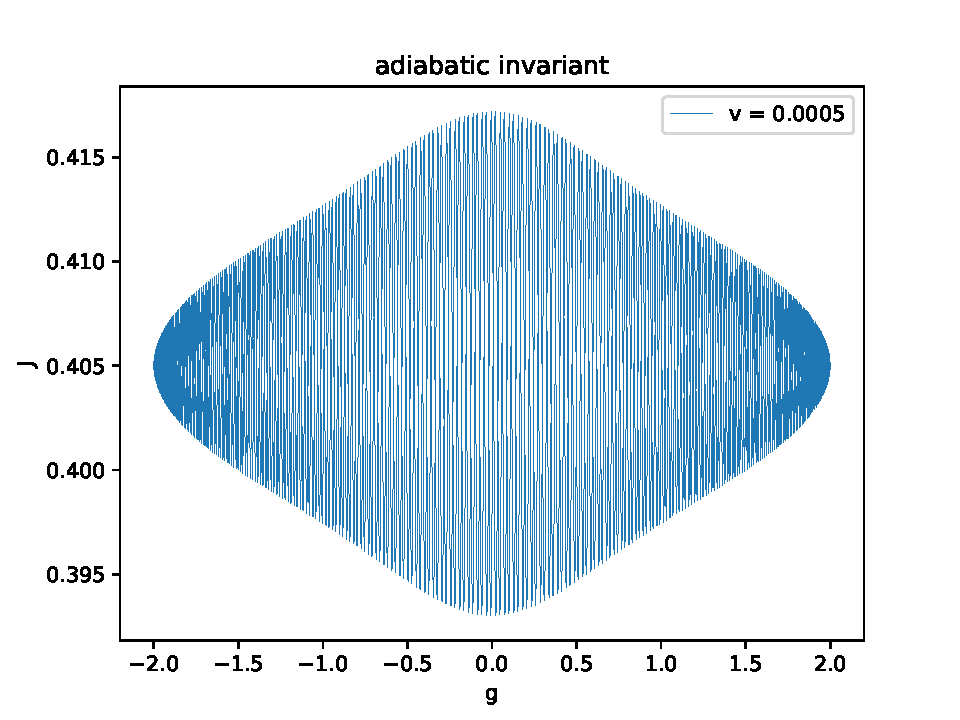
\includegraphics[scale=0.6]{4g_ad_invr_v=0_0005.pdf}
        \caption{绝热不变量随$g$的变化}
        \label{4 g ad}
    \end{figure}
    \begin{figure}[htbp]
        \centering
        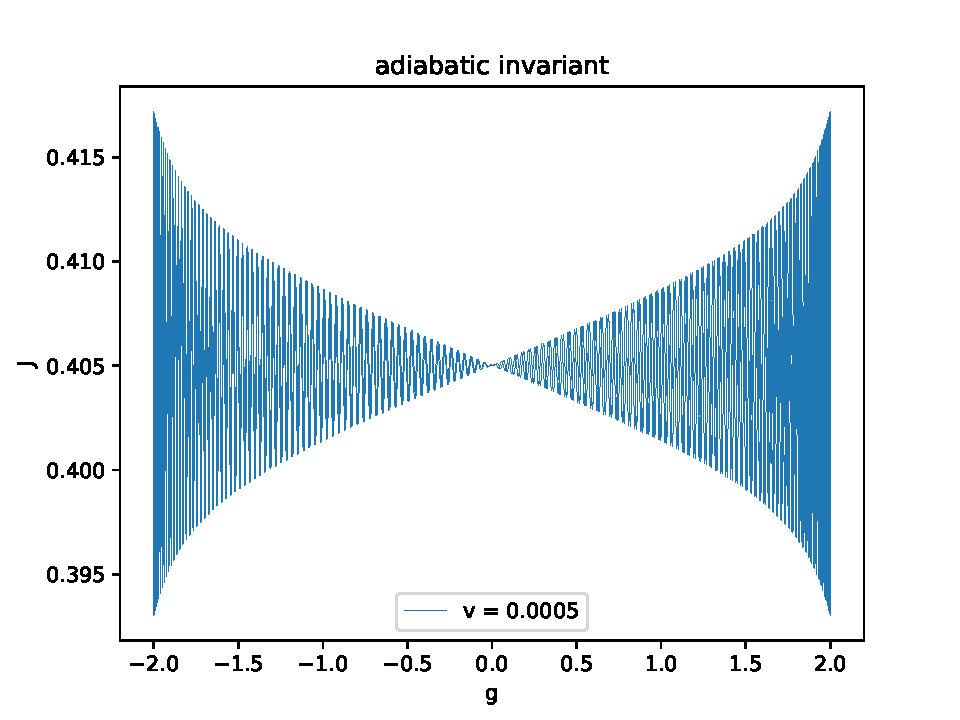
\includegraphics[scale=0.6]{4x_ad_invr_v=0_0005.pdf}
        \caption{绝热不变量随$x$的变化}
        \label{4 x ad}
    \end{figure}
    \par 
    计算得到的Berry相位为$\phi_B = -0.00199$, 可以认为等于0. 
    \subsubsection{问题(5)}
    由于这一问中外参数变化不如前一问剧烈, 因此将参数选择为较大的$\nu=0.001$, 演化过程中的轨线、绝热不变量随参数的变化可以参见图
    \begin{figure}[htbp]
        \centering
        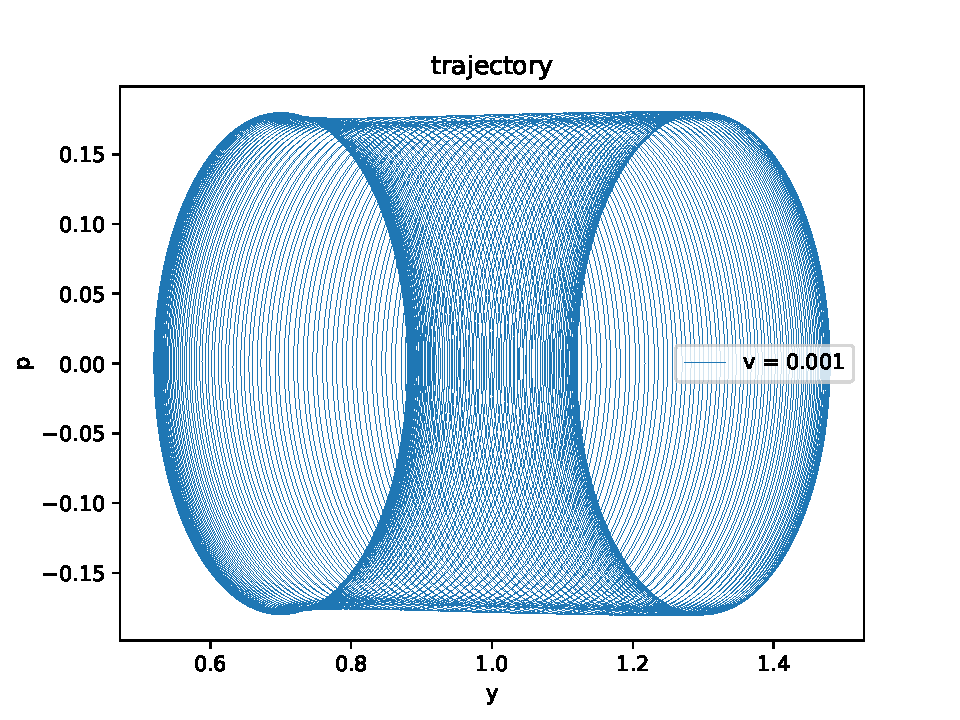
\includegraphics[scale=0.6]{5_traj_v=0_001.pdf}
        \caption{参数变化一个周期时相空间轨线}
        \label{5 traj}
    \end{figure}
    \begin{figure}[htbp]
        \centering
        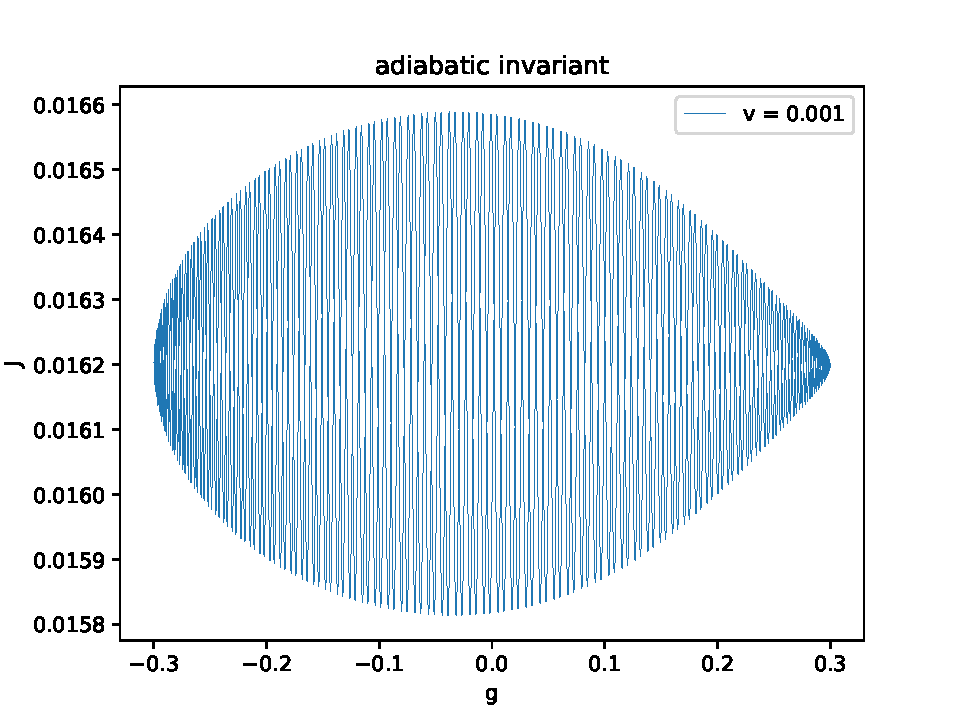
\includegraphics[scale=0.6]{5g_ad_invr_v=0_001.pdf}
        \caption{绝热不变量随$g$的变化}
        \label{5 g ad}
    \end{figure}
    \begin{figure}[htbp]
        \centering
        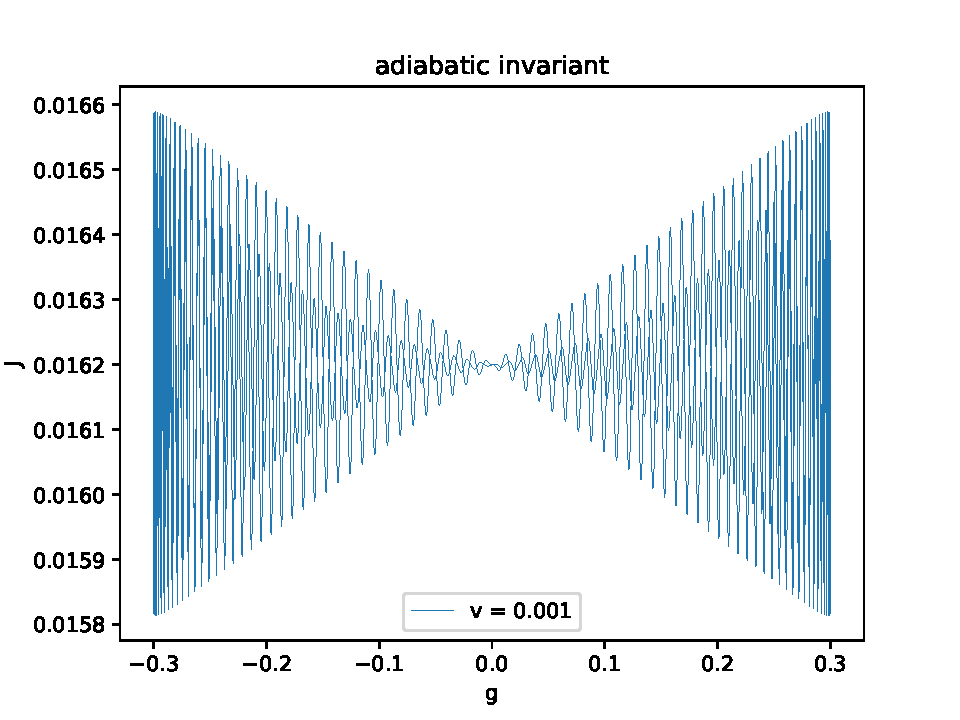
\includegraphics[scale=0.6]{5x_ad_invr_v=0_001.pdf}
        \caption{绝热不变量随$x$的变化}
        \label{5 x ad}
    \end{figure}
    \par 
    计算得到的Berry相位为$\phi_B = -0.0055$, 偏差比前一问略大, 或许真的应该选取小一点的$\nu$. 观察轨线还可以发现, 
    这一问给的初始条件能量比较小, 不足以系统跨越中心的势垒, 因此只能在某一侧的势阱中跟随着势阱的极小值点变化不断运动.
\end{document}